\documentclass[journal]{IEEEtran}
\usepackage{amsmath,amssymb,amsfonts}
\usepackage{algorithmic}
\usepackage{algorithm}
\usepackage{array}
\usepackage{textcomp}
\usepackage{stfloats}
\usepackage{url}
\usepackage{verbatim}
\usepackage{graphicx}
\usepackage{cite}
\usepackage{booktabs}
\usepackage{multirow}
\usepackage{balance}

\hyphenation{op-tical net-works semi-conduc-tor IEEE-Xplore}

\begin{document}

\title{Intent-Aware Multi-Agent Cognitive Swarm Intelligence (I-MACSI) for Autonomous Mission-Driven Self-Organization in AI-Native LEO Mega-Constellation Networks}

\author{
    \IEEEauthorblockN{Anonymous Author(s)}\\
    \IEEEauthorblockA{\textit{Affiliation and institutional details omitted for double-blind peer review}}\\
    \textit{Manuscript submitted for journal review --- October 2026}
}

\markboth{Research Manuscript Under Peer Review --- Anonymized Submission Draft, October 2026}%
{I-MACSI: Intent-Aware Multi-Agent Cognitive Swarm Intelligence for LEO Networks}

\maketitle

\begin{abstract}
Future Low Earth Orbit (LEO) satellite mega-constellations deployed in sixth-generation (6G) Space-Air-Ground Integrated Networks (SAGIN) must concurrently support highly heterogeneous missions---spanning ultra-reliable low-latency disaster telemetry, high-throughput Earth observation downlinks, military tactical reconnaissance, and broadband internet. Conventional routing architectures, including Dijkstra-based shortest-path and unshaped Multi-Agent Reinforcement Learning (MARL), optimize uniform network indicators (propagation delay or queue occupancy) without recognizing the semantic intent of underlying missions. During space radiation outages or orbital bottleneck congestion, critical missions are frequently starved in favor of bulk background traffic. To resolve this paradigm limitation, this paper proposes I-MACSI (Intent-Aware Multi-Agent Cognitive Swarm Intelligence), an autonomous self-organizing framework that shifts satellite mega-constellations from traffic-aware to mission-aware. I-MACSI introduces: (i) an 8-dimensional normalized Mission Intent Vector (MIV) encoding latency, throughput, reliability, congestion, energy, security, coverage, and compute requirements; (ii) a bounded gossip dissemination protocol ($TTL=2$) incurring less than 0.05\% ISL signaling overhead; (iii) decentralized multi-agent Q-routing with dynamically shaped Bellman rewards; (iv) federated swarm consensus for distributed Q-table synchronization; and (v) a post-routing joint resource optimizer governing link bandwidth, beam steering, compute offloading, and Earth gateway selection. A rigorous empirical evaluation benchmarking I-MACSI against nine state-of-the-art baselines across 77 comprehensive metrics with 95\% confidence intervals demonstrates that I-MACSI achieves 24.56~Gbps throughput (+26.6\% vs. MADRL), maintains 28.01~ms end-to-end latency (-22.3\% vs. MADRL), preserves 97.4\% priority satisfaction for mission-critical traffic, and sustains 86.0\% packet delivery ratio under 30\% inter-satellite link severance.
\end{abstract}

\begin{IEEEkeywords}
Low Earth Orbit (LEO) Mega-Constellations, Intent-Based Networking (IBN), Multi-Agent Reinforcement Learning (MARL), Cognitive Swarm Intelligence, Inter-Satellite Links (ISL), Autonomous Self-Healing, 6G SAGIN.
\end{IEEEkeywords}

\section{Introduction}
\IEEEPARstart{T}{he} explosive commercial and scientific expansion of Low Earth Orbit (LEO) mega-constellations---typified by constellations such as SpaceX Starlink, Amazon Project Kuiper, Eutelsat OneWeb, and China's Guowang (GW)---marks a fundamental architectural paradigm shift in global telecommunications. Operating at orbital altitudes between 500~km and 1,500~km, LEO networks deliver low propagation latency and global visibility unattainable by legacy Geostationary Earth Orbit (GEO) satellites. In emerging sixth-generation (6G) Space-Air-Ground Integrated Network (SAGIN) visions, LEO constellations serve as the spaceborne backbone for massive Internet-of-Things (IoT), remote autonomous maritime navigation, military tactical reconnaissance, disaster emergency response, and edge cloud telemetry~\cite{akyildiz2005wireless, zhang20196g}.

Despite their vast spatial capacity, operational LEO mega-constellations operate under extreme physical and topological constraints. Traveling at orbital velocities of approximately 7.5~km/s, satellites undergo continuous orbital motion, causing periodic line-of-sight variations, rapid Doppler frequency shifts, and brief contact windows with Earth ground stations. Inter-Satellite Links (ISLs)---primarily free-space optical (FSO) laser links and millimeter-wave (mmWave) cross-links---suffer severe pointing, acquisition, and tracking (PAT) disruptions during polar crossings and orbital plane crossings. Furthermore, high space-radiation flux and micrometeoroid encounters periodically degrade transceiver electronics, precipitating sudden link outages~\cite{kaushal2017optical, cheng2019space}.

\subsection{Research Gap}
Conventional satellite routing strategies remain fundamentally traffic-blind. Legacy algorithms such as Dijkstra's shortest path, Open Shortest Path First (OSPF), and Equal-Cost Multi-Path (ECMP) treat every packet as an undifferentiated bitstream, routing solely based on instantaneous physical distance or static hop counts~\cite{dijkstra1959note}. While recent advances have explored Multi-Agent Deep Reinforcement Learning (MADRL) and Graph Neural Networks (GNNs) for distributed space routing~\cite{wang2021multi, chen2022graph}, existing learning formulations rely on rigid, universal reward functions (e.g., minimizing average queue delay). Consequently, during high orbital traffic congestion or catastrophic link severances, mission-critical emergency telemetry (demanding ultra-low latency and zero packet loss) competes on equal terms with delay-tolerant background Earth observation data (demanding massive throughput), leading to catastrophic mission failure.

\subsection{Contributions}
To overcome these foundational limitations, this paper proposes \textbf{I-MACSI} (Intent-Aware Multi-Agent Cognitive Swarm Intelligence), an autonomous self-organizing networking framework that enables semantic mission-driven routing and distributed resource management in AI-native LEO constellations. The major contributions of this work are summarized as follows:
\begin{enumerate}
    \item \textbf{Unified 8-Dimensional Mission Intent Model:} We formulate a normalized Mission Intent Vector (MIV) that captures latency, throughput, reliability, congestion, energy, security, geographic coverage, and computational demands, bridged by a semantic natural language intent parser.
    \item \textbf{Bounded-Overhead Intent Dissemination:} We design a localized gossip dissemination protocol with Time-To-Live ($TTL = 2$) that limits control message overhead to less than 0.05\% of optical ISL bandwidth while ensuring swarm-wide regional mission awareness.
    \item \textbf{Adaptive Semantic Reward Shaping in MARL:} We integrate mission intent weights directly into the local Bellman equation of satellite agents, allowing decentralized Q-routing tables to dynamically adapt their decision boundaries to operational priorities.
    \item \textbf{Decentralized Federated Swarm Consensus:} We implement an inter-satellite consensus mechanism wherein adjacent orbital nodes periodically average Q-tables and merge intent caches, achieving resilient swarm coordination without centralized ground intervention.
    \item \textbf{Post-Routing Joint Resource Graph Optimization:} We develop a joint optimization layer that coordinates ISL bandwidth allocation, dynamic beam steering, compute offloading, and Earth feeder gateway selection along routed mission paths.
    \item \textbf{Comprehensive 77-Metric Empirical Benchmark:} We benchmark I-MACSI against nine state-of-the-art baselines across 77 empirical metrics with 95\% confidence intervals across 50 Monte Carlo trials, accompanied by formal paired t-tests, Wilcoxon signed-rank tests, and Cohen's $d$ effect sizes.
\end{enumerate}

\section{Related Work and Literature Comparison}
Satellite routing research has evolved from static topological tables to dynamic, learning-driven architectures. Early landmark works adopted virtual topology models and discrete-time snapshot techniques to accommodate deterministic orbital motions~\cite{henderson2000distributed}. However, snapshot methods cannot absorb stochastic link disruptions or transient congestion hotspots. Reinforcement learning (RL) was first adapted to packet networks via Boyan and Littman's Q-routing~\cite{boyan1994packet}, demonstrating local adaptation but suffering from slow exploration in high-diameter constellations.

With the advent of deep learning, Multi-Agent Deep Reinforcement Learning (MADRL) models utilizing Centralized Training with Decentralized Execution (CTDE), such as MADDPG~\cite{lowe2017multi} and MAPPO~\cite{yu2022surprising}, were applied to satellite mega-constellations~\cite{sheng2022hierarchical}. Graph Reinforcement Learning (Graph RL) and Graph Attention Networks (GAT-RA)~\cite{almasan2022deep, velickovic2018graph} further incorporated topology embeddings to handle dynamic spatial graph variations. Concurrently, Federated MARL (FedMARL)~\cite{mcmahan2017communication} explored privacy-preserving distributed model aggregation. In terrestrial Software-Defined Networks (SDNs), Intent-Based Networking (IBN, formalized in IETF RFC 9315)~\cite{rfc9315} demonstrated the translation of declarative business intents into network policies. However, extending centralized IBN controllers to space is severely impeded by the 50--150~ms ground-satellite propagation delay. Table~\ref{tab:literature} provides a comprehensive comparative analysis of existing paradigms and contrasts them with the proposed I-MACSI framework.

\begin{table*}[t]
\centering
\caption{Detailed Comparative Analysis of Existing Works and Proposed I-MACSI Framework}
\label{tab:literature}
\resizebox{\textwidth}{!}{%
\begin{tabular}{p{3.2cm}p{2.5cm}p{3.2cm}p{2.5cm}p{2.5cm}p{4cm}p{4.2cm}}
\toprule
\textbf{Algorithmic Family / Ref.} & \textbf{Control Architecture} & \textbf{Learning / Optimization Core} & \textbf{Semantic Intent Awareness} & \textbf{Dynamic Fault Recovery} & \textbf{Primary Architectural Limitation} & \textbf{Distinction of Proposed I-MACSI} \\
\midrule
Shortest Path (Dijkstra)~\cite{dijkstra1959note} & Centralized / Distributed & Graph Dijkstra / SPF & None (Static Metric) & Reactive / Re-flooding & Severe congestion; ignores mission SLA & Dynamic 8D intent-shaped multi-agent cost \\
Classical Q-Routing~\cite{boyan1994packet} & Distributed & Tabular Bellman Q-Learning & None (Delay Only) & Local Q-table update & Unshaped scalar reward; slow convergence & Intent-shaped reward with federated consensus \\
MADRL (MAPPO/MADDPG)~\cite{lowe2017multi, sheng2022hierarchical} & CTDE (Hybrid) & Deep Actor-Critic PPO/DDPG & Rigid Global Reward & Policy re-evaluation & High compute footprint; ignores mission semantics & Lightweight tabular swarm with intent vector \\
Graph RL~\cite{almasan2022deep} & Decentralized & GNN + Deep Q-Network & None (Topology Only) & Graph message passing & Heavy matrix multiplication; GPU dependent & Decentralized graph walk on spaceborne CPU \\
H-MARL~\cite{sheng2022hierarchical} & Hierarchical & Two-tier Meta/Worker RL & Coarse Sub-goals & Hierarchical delegation & Slow inter-tier coordination latency & Flat peer-to-peer cognitive swarm intelligence \\
GAT-RA~\cite{velickovic2018graph} & Centralized / Cluster & Graph Attention Networks & Implicit QoS Weights & Attention re-weighting & High compute complexity $\mathcal{O}(|\mathcal{V}|^2)$ & Lightweight gossip consensus $\mathcal{O}(\Delta^2)$ \\
FedMARL~\cite{mcmahan2017communication} & Federated Decentralized & FedAvg Model Aggregation & None (Generic Policy) & Federated consensus & Optimizes purely for network-level metrics & FedMARL enhanced by semantic intent caching \\
Intent-Based Networking~\cite{rfc9315} & Centralized SDN & Policy Compiler / Global SPF & Declarative Rule-Based & Controller recomputation & Single point of failure; 50--150~ms ground latency & Fully autonomous in-orbit swarm self-healing \\
Semantic Comm.~\cite{qin2021semantic} & Point-to-Point & Deep Autoencoder / NLP & Payload Semantic Comp. & End-to-end retraining & Payload compression only; no network routing & Network-wide multi-agent routing optimization \\
\midrule
\textbf{Proposed I-MACSI} & \textbf{Decentralized Swarm} & \textbf{8D Intent MARL + FedMARL} & \textbf{Full 8D Intent Vector} & \textbf{Instant Autonomous Swarm} & \textbf{---} & \textbf{Unifies semantic intent, decentralized MARL, federated consensus \& resource slicing} \\
\bottomrule
\end{tabular}%
}
\end{table*}

\section{LEO Mega-Constellation System Model}
\subsection{Orbital Topology and Adjacency}
Consider a Walker-delta or Walker-star LEO mega-constellation modeled as a time-varying directed graph $\mathcal{G}(t) = (\mathcal{V}, \mathcal{E}(t))$, where $\mathcal{V}$ denotes the set of $|\mathcal{V}|$ satellite nodes and $\mathcal{E}(t)$ represents active Inter-Satellite Links (ISLs) at time $t$. The constellation comprises $P$ orbital planes with $S$ satellites per plane ($|\mathcal{V}| = P \times S$). Each satellite $i$ is uniquely identified by its orbital coordinates $(p, s)$, where $p \in \{0, \dots, P-1\}$ and $s \in \{0, \dots, S-1\}$. Under nominal geometry, each satellite maintains four bidirectional ISLs: two intra-plane links to adjacent satellites $(p, (s \pm 1) \bmod S)$ with distance $d_{\text{intra}} = 1500$~km, and two inter-plane links to cross-plane neighbors $((p \pm 1) \bmod P, s)$ with distance $d_{\text{inter}} = 2500$~km.

\subsection{Physical ISL Latency and Queueing}
Over an active ISL $e = (u, v) \in \mathcal{E}(t)$ with physical length $d_e$, the instantaneous packet latency $\tau_e(t)$ incorporates free-space propagation delay, queueing delay, stochastic jitter, cryptographic security overhead, and an operational state multiplier $\mu_{\text{state},e}(t) \in \{1.0, 1.5, \infty\}$:
\begin{equation}
\tau_e(t) = \mu_{\text{state},e}(t) \cdot \left[ \frac{d_e}{c} + \tau_{\text{queue},e}(t) + \delta_{\text{jitter}} + \tau_{\text{enc},e}(t) \right]
\label{eq:latency}
\end{equation}
where $c = 3.0 \times 10^5$~km/s ($300$~km/ms) is the optical velocity of light. Queueing delay $\tau_{\text{queue},e}(t)$ is governed by link utilization factor $U_e(t) = \min(\lambda_e(t) / C_{\max}, 0.99)$ under an $M/M/1$-equivalent queueing model with base packet service time $\tau_0 = 2.0$~ms and dynamic congestion penalty $\psi_{\text{cong},e}(t) \in [0, 1]$:
\begin{equation}
\tau_{\text{queue},e}(t) = \left[ \frac{U_e(t)}{1 - U_e(t)} \right] \cdot \tau_0 \cdot \left(1.0 + \psi_{\text{cong},e}(t)\right)
\label{eq:queue}
\end{equation}
For encrypted transmission (AES-GCM-256 link encryption enforced on defense missions), the encryption overhead is $\tau_{\text{enc},e}(t) = 0.5 + 1.5 \psi_{\text{cong},e}(t)$~ms, whereas $\tau_{\text{enc}} = 0$ for standard unencrypted traffic.

\subsection{Packet Loss and Link Reliability}
The total packet loss probability $p_{\text{loss},e}(t)$ incorporates baseline space channel loss $p_{\text{base}} = 0.001$, link state impairment loss $p_{\text{state},e}$, congestion loss, and buffer overflow loss:
\begin{equation}
p_{\text{loss},e}(t) = \min\left( 1.0, \, p_{\text{base}} + p_{\text{state},e}(t) + 0.2 \psi_{\text{cong},e}(t) + 0.05 \max(0, U_e(t) - 0.8) \right)
\label{eq:loss}
\end{equation}
where $p_{\text{state}} = 0.15$ for DEGRADED links, $0.05$ for RECOVERING links, and $1.0$ for FAILED links. Link reliability is defined as $R_e(t) = 1.0 - p_{\text{loss},e}(t)$. Available bandwidth is expressed as $C_{\text{avail},e}(t) = \max(0, C_{\max} - \lambda_e(t)) \cdot (1 - \psi_{\text{cong},e}(t))$ for active links and 0 for failed links.

\subsection{Energy Consumption}
Transmit energy per packet over ISL $e$ is proportional to RF/optical transmit power $P_{\text{tx}}$ and propagation duration: $E_e = 10^{(P_{\text{tx}} - 30)/10} \cdot (d_e / c) \cdot 1000$~mJ.

\begin{table}[b]
\centering
\caption{System Model Parameters and Mathematical Notations}
\label{tab:notations}
\resizebox{\columnwidth}{!}{%
\begin{tabular}{lll}
\toprule
\textbf{Symbol} & \textbf{Mathematical Definition} & \textbf{Default Value / Units} \\
\midrule
$\mathcal{G}(t) = (\mathcal{V}, \mathcal{E}(t))$ & Time-varying LEO constellation network graph & $|\mathcal{V}| \in [20, 200]$ nodes \\
$P, S$ & Orbital planes and satellites per plane & $P \times S = |\mathcal{V}|$ (e.g., $4\times 4, 10\times 10$) \\
$d_{\text{intra}}, d_{\text{inter}}$ & Intra-plane and inter-plane physical link distances & 1,500~km / 2,500~km \\
$c$ & Free-space propagation velocity of optical ISL & $3.0 \times 10^5$~km/s ($300$~km/ms) \\
$C_{\max}$ & Maximum physical optical ISL transmission capacity & 1,000~Mbps (1.0~Gbps) \\
$\tau_e(t)$ & Total instantaneous one-hop ISL latency & Milliseconds (ms) \\
$U_e(t)$ & Link utilization factor ($\lambda_e / C_{\max}$) & Dimensionless, in $[0.0, 0.99]$ \\
$\psi_{\text{cong},e}(t)$ & Localized buffer congestion penalty level & Dimensionless, in $[0.0, 1.0]$ \\
$I_m$ & 8-Dimensional normalized Mission Intent Vector & Normalized $\sum w_i = 1.0$ \\
$\pi_m$ & Operational mission priority tier & Integer scale $[1, 10]$ \\
$\alpha, \gamma$ & Learning rate and discount factor for Q-routing & $\alpha = 0.1, \gamma = 0.9$ \\
$TTL$ & Time-To-Live for bounded intent gossip dissemination & $TTL = 2$ hops \\
$w_{\text{cons}}$ & Federated swarm consensus weighting coefficient & $w_{\text{cons}} = 0.2$ \\
$T_{\text{sync}}$ & Periodic consensus synchronization interval & 20 simulation ticks \\
\bottomrule
\end{tabular}%
}
\end{table}

\section{Mission Intent Representation and Problem Formulation}
\subsection{8-Dimensional Mission Intent Vector}
In contrast to conventional scalar QoS parameters, I-MACSI formalizes mission semantics through an 8-dimensional normalized Mission Intent Vector (MIV):
\begin{equation}
I_m = [ w_{\text{lat}}, w_{\text{thr}}, w_{\text{rel}}, w_{\text{cong}}, w_{\text{egy}}, w_{\text{sec}}, w_{\text{cov}}, w_{\text{comp}} ]^T
\label{eq:intent_vec}
\end{equation}
subject to $\sum_{k=1}^8 w_k = 1.0$, with $w_k \ge 0$, and operational priority tier $\pi_m \in \{1, \dots, 10\}$.

\subsection{Normalized Intent-Aware Link Cost Function}
For an ISL $e = (u, v)$, the normalized base cost $c_e(I_m)$ is computed as:
\begin{equation}
c_e(I_m) = \frac{1}{\pi_m} \sum_{k=1}^8 w_k P_{k,e}
\label{eq:cost}
\end{equation}
where normalized penalty dimensions $P_{k,e} \in [0, 1]$ are defined as:
\begin{align}
P_{\text{lat},e} &= \min(\tau_e / \tau_{\max}, 1.0) \\
P_{\text{thr},e} &= 1.0 - \min(C_{\text{avail},e} / C_{\max}, 1.0) \\
P_{\text{rel},e} &= \min(p_{\text{loss},e} + (1.0 - R_{\text{intrinsic}}), 1.0) \\
P_{\text{cong},e} &= \min(\psi_{\text{cong},e}, 1.0) \\
P_{\text{egy},e} &= \min(E_e / E_{\max}, 1.0) \\
P_{\text{sec},e} &= (0.0\text{ if encrypted else }1.0) \times 0.8 + \min(\tau_{\text{enc}} / 2.0, 1.0) \times 0.2 \\
P_{\text{cov},e} &= 1.0 - \min(\tau_e / \tau_{\max}, 1.0) \\
P_{\text{comp},e} &= \min(1.2 \psi_{\text{cong},v}, 1.0)
\end{align}
If link $e$ is in state FAILED, $c_e(I_m) = \infty$.

\subsection{Constrained Multi-Objective Routing Formulation}
The global mission routing problem for flow $m$ from source $s_m$ to destination $d_m$ is formulated as finding path $\mathcal{P}_m^* = (v_0, v_1, \dots, v_K)$ minimizing total intent cost subject to operational constraints:
\begin{align}
\min_{\mathcal{P}_m} \quad & \sum_{e \in \mathcal{P}_m} c_e(I_m) \label{eq:obj} \\
\text{s.t.} \quad & \sum_{e \in \mathcal{P}_m} \tau_e(t) \le \tau_{\text{deadline},m} \label{eq:c_lat} \\
& \min_{e \in \mathcal{P}_m} C_{\text{avail},e}(t) \ge R_{\text{demand},m} \label{eq:c_bw} \\
& \prod_{e \in \mathcal{P}_m} (1 - p_{\text{loss},e}(t)) \ge \rho_{\text{rel},m} \label{eq:c_rel} \\
& P_{\text{sec},e} = 0, \quad \forall e \in \mathcal{P}_m, \quad \text{if } w_{\text{sec},m} \ge 0.3 \label{eq:c_sec}
\end{align}

\subsection{Complexity and NP-Hardness}
The multi-constrained path problem defined by (\ref{eq:obj})--(\ref{eq:c_sec}) is a Multi-Constrained Optimal Path (MCOP) problem, known to be strictly NP-hard when subject to two or more additive non-correlated constraints (latency and packet loss). In an operational LEO constellation with dynamic ISLs, solving (\ref{eq:obj})--(\ref{eq:c_sec}) via centralized integer linear programming is computationally intractable and introduces unacceptable signaling delay, motivating the decentralized multi-agent cognitive swarm solution of I-MACSI.

\section{The Proposed I-MACSI Framework}
\subsection{Cognitive Swarm Architecture}
I-MACSI executes as a distributed cognitive swarm where each satellite acts as an autonomous reinforcement learning agent. The decision pipeline comprises four interlocking mechanisms:

\subsubsection{Bounded Gossip Dissemination ($TTL = 2$)}
Upon receiving a mission flow, the source satellite extracts $I_m$ via keyword semantic mapping and broadcasts a lightweight intent descriptor to its direct 1-hop and 2-hop neighbors. Dissemination is strictly bounded by $TTL = 2$ with duplicate sequence filtering, guaranteeing that intent signaling remains confined to $\mathcal{O}(\Delta^2)$ messages (where $\Delta \le 4$ is the constellation node degree) and consumes less than 0.05\% of optical link bandwidth.

\subsubsection{Dynamic Bellman Reward Shaping}
Each satellite node $u$ maintains a local Q-table $Q_u(I_m, d, v)$, representing the estimated cumulative cost of forwarding a packet destined for $d$ with active intent $I_m$ to neighbor $v \in \text{Adj}(u)$. When forwarding occurs, node $u$ updates $Q$ via dynamic reward shaping:
\begin{equation}
Q_u(I_m, d, v) \leftarrow (1 - \alpha) Q_u(I_m, d, v) + \alpha \left[ c_{\text{shaped},e}(I_m) + \gamma \min_{v'} Q_v(I_m, d, v') \right]
\label{eq:q_update}
\end{equation}
where dynamic reward shaping modulates cost based on intent bonuses and penalties:
\begin{equation}
c_{\text{shaped},e}(I_m) = \max\left(0.0, \, c_e(I_m) - \Delta_{\text{intent}}(I_m)\right)
\label{eq:shaped_cost}
\end{equation}
\begin{equation}
\Delta_{\text{intent}}(I_m) = 0.05 w_{\text{sec}} \mathbf{1}_{\{\text{encrypted}\}} - 0.03 w_{\text{egy}} + 0.04 w_{\text{comp}} + 0.03 w_{\text{cov}}
\end{equation}
If priority $\pi_m \ge 8$, the shaped cost is amplified by 1.15 to accelerate learning for critical flows. If an ISL fails, a catastrophic penalty $\Lambda_{\text{fail}} = 1000.0$ is applied. If a routing loop is detected, $\Lambda_{\text{loop}} = 500.0$ is penalized, ensuring rapid loop breaking.

\subsubsection{Federated Swarm Consensus}
To accelerate convergence across orbital planes without centralized coordination, satellite nodes execute periodic federated averaging (FedMARL) every $T_{\text{sync}} = 20$ steps:
\begin{equation}
Q_u(I_m, d, v) \leftarrow (1 - w_{\text{cons}}) Q_u(I_m, d, v) + w_{\text{cons}} \frac{1}{|\mathcal{N}_{\text{active}}(u)|} \sum_{k \in \mathcal{N}_{\text{active}}(u)} Q_k(I_m, d, v)
\label{eq:consensus}
\end{equation}

\subsubsection{Post-Routing Joint Resource Graph Optimization}
Once a packet's path $\mathcal{P}_m$ is established, a greedy graph-walk optimizer allocates dynamic link bandwidth slices $C_{\text{alloc}} = \min(C_{\text{avail}}, B_{\text{req}}(I_m))$, triggers phased-array beam hopping on intermediate nodes, offloads compute tasks to the satellite on $\mathcal{P}_m$ with the minimum computational load, and designates the optimal Earth gateway downlink at the first or last orbital plane.

\subsubsection{Autonomous Self-Healing and Topology Reorganization}
When an ISL fails, the detecting satellite immediately sets $Q_u(\cdot, \cdot, v_{\text{failed}}) = \Lambda_{\text{fail}}$, decays adjacent Q-values, and triggers a localized reroute along the second-best neighbor, achieving autonomous self-healing within milliseconds without waiting for ground telecommand. Algorithm~\ref{algo:imacsi} summarizes the complete operational procedure.

\begin{algorithm}[t]
\caption{I-MACSI End-to-End Cognitive Swarm Execution Pipeline}
\label{algo:imacsi}
\begin{algorithmic}[1]
\REQUIRE Constellation graph $\mathcal{G}(t)=(\mathcal{V}, \mathcal{E}(t))$; Mission request with intent; $\alpha=0.1, \gamma=0.9, w_{\text{cons}}=0.2$.
\ENSURE Optimal intent-guided routing path $\mathcal{P}_m^*$; Resource allocation plan; Updated Q-tables.
\STATE \textbf{Phase I: Intent Extraction \& Bounded Gossip Dissemination}
\STATE Extract 8D Intent Vector $I_m = [w_{\text{lat}}, \dots, w_{\text{comp}}]$ via keyword semantic engine; Normalize $\sum w_i = 1.0$; Assign priority tier $\pi_m \in [1, 10]$.
\STATE Broadcast intent descriptor to 1-hop and 2-hop neighbors via gossip protocol with $TTL=2$; update neighborhood intent caches.
\STATE \textbf{Phase II: Multi-Agent Intent-Aware Q-Routing}
\STATE Initialize current node $u = s_m$, Path $\mathcal{P}_m = [s_m]$, Hop count $h = 0$.
\WHILE{$u \ne d_m$ \AND $h < \text{Max\_Hops}$}
    \STATE Query candidate neighbors $v \in \text{Adj}(u)$ with active ISL state $\ne \text{FAILED}$.
    \STATE With probability $(1 - \epsilon)$, select next hop $v^* = \arg\min_v Q_u(I_m, d_m, v)$; else explore random neighbor.
    \STATE Compute instantaneous link metrics: latency $\tau_e$, loss $p_{\text{loss}}$, energy $E_e$, encryption status.
    \STATE Calculate 8D intent cost $c_e(I_m)$ via (\ref{eq:cost}) and shaped cost $c_{\text{shaped},e}(I_m)$ via (\ref{eq:shaped_cost}).
    \STATE Execute Bellman policy update on node $u$ via (\ref{eq:q_update}); Append $v^*$ to $\mathcal{P}_m$; Advance $u \leftarrow v^*$; $h \leftarrow h + 1$.
\ENDWHILE
\STATE \textbf{Phase III: Post-Routing Joint Resource Graph Optimization}
\STATE Compute bottleneck bandwidth along $\mathcal{P}_m$ and slice bandwidth allocation.
\STATE Activate phased-array beam steering on intermediate nodes; Offload compute task to $\arg\min_{k \in \mathcal{P}_m} L_{\text{comp}}(k)$.
\STATE Assign feeder gateway downlink to terminal orbital boundary node ($p=0$ or $p=P-1$).
\STATE \textbf{Phase IV: Periodic Swarm Consensus \& Self-Healing}
\IF{$\text{current\_step} \bmod T_{\text{sync}} == 0$}
    \STATE Synchronize Q-tables and intent caches across active neighbors using federated consensus (\ref{eq:consensus}).
\ENDIF
\IF{link failure detected on $e=(u, v)$}
    \STATE Apply $Q_u(\cdot, \cdot, v) \leftarrow \Lambda_{\text{fail}}$; execute localized detour reroute.
\ENDIF
\end{algorithmic}
\end{algorithm}

\section{Simulation Results and Empirical Evaluation}
\subsection{Simulation Environment and Setup}
The evaluation environment was implemented in Python 3.13 utilizing NetworkX, NumPy, and Matplotlib, interfaced with discrete-event orbital simulators. The constellation size was swept from 20 to 200 satellites arranged in Walker-delta geometry, handling concurrent user loads ranging from 100 to 5,000 active sessions across ten standard mission profiles. All experimental curves report mean values and 95\% confidence intervals derived from 50 independent Monte Carlo trials ($t_{\text{crit}} = 2.0096$). Table~\ref{tab:sim_params} lists the simulation parameters.

\begin{table}[h]
\centering
\caption{Simulation Environment and Benchmark Parameters}
\label{tab:sim_params}
\resizebox{\columnwidth}{!}{%
\begin{tabular}{lll}
\toprule
\textbf{Simulation Parameter} & \textbf{Empirical Value / Range} & \textbf{Physical Operational Context} \\
\midrule
Constellation Scale ($|\mathcal{V}|$) & 20 to 200 satellites (swept) & Walker-delta LEO mega-constellation \\
Orbital Altitude ($h$) & 550~km (nominal LEO) & Low Earth Orbit space environment \\
Active Traffic Flows & 10 to 200 concurrent flows per batch & Mixed mission intent profiles \\
User Scaling Range & 100 to 5,000 users & Massive IoT \& broadband demand \\
ISL Physical Capacity ($C_{\max}$) & 1,000~Mbps (1~Gbps) & Optical laser cross-link bandwidth \\
Link Failure Probability & 0\% to 50\% link severance (swept) & Space radiation \& debris stress \\
Satellite Outage Probability & 0\% to 25\% satellite node failure & Onboard payload power blackout \\
Learning Hyperparameters & $\alpha = 0.1, \gamma = 0.9, \epsilon_0 = 0.1$ & Decentralized Q-learning engine \\
Consensus Weight / Sync & $w_{\text{cons}} = 0.2, T_{\text{sync}} = 20$ steps & Federated swarm Q-table consensus \\
Monte Carlo Sample Size & $N = 50$ runs per data point & 95\% CI error bar estimation ($t_{\text{crit}}=2.01$) \\
\bottomrule
\end{tabular}%
}
\end{table}

\subsection{Communication Performance Under Constellation Scaling}
Figures~\ref{fig:tp} and~\ref{fig:lat} evaluate communication throughput and end-to-end packet latency as constellation size scales from 20 to 200 satellites. As the number of satellites expands, spatial mesh diversity increases, providing more concurrent alternate paths. I-MACSI consistently achieves the highest aggregate throughput across all scales, reaching 24.56~Gbps at $|\mathcal{V}| = 200$ satellites (+26.6\% over MADRL, +54.5\% over centralized IBN, and +142.7\% over Dijkstra). This performance advantage arises from I-MACSI's intent-driven traffic distribution: bulk Earth observation flows are steered toward wide-aperture high-capacity cross-links, preventing bottleneck saturation on primary paths. In contrast, Dijkstra and centralized IBN funnel traffic onto identical shortest paths, inducing severe buffer bloat. Similarly, I-MACSI limits end-to-end latency to 28.01~ms at 100 satellites (a 22.3\% reduction vs. MADRL and 50.9\% vs. IBN) by enforcing latency penalties in Q-routing for time-critical flows.

\begin{figure*}[t]
\centering
\begin{minipage}{0.48\textwidth}
\centering
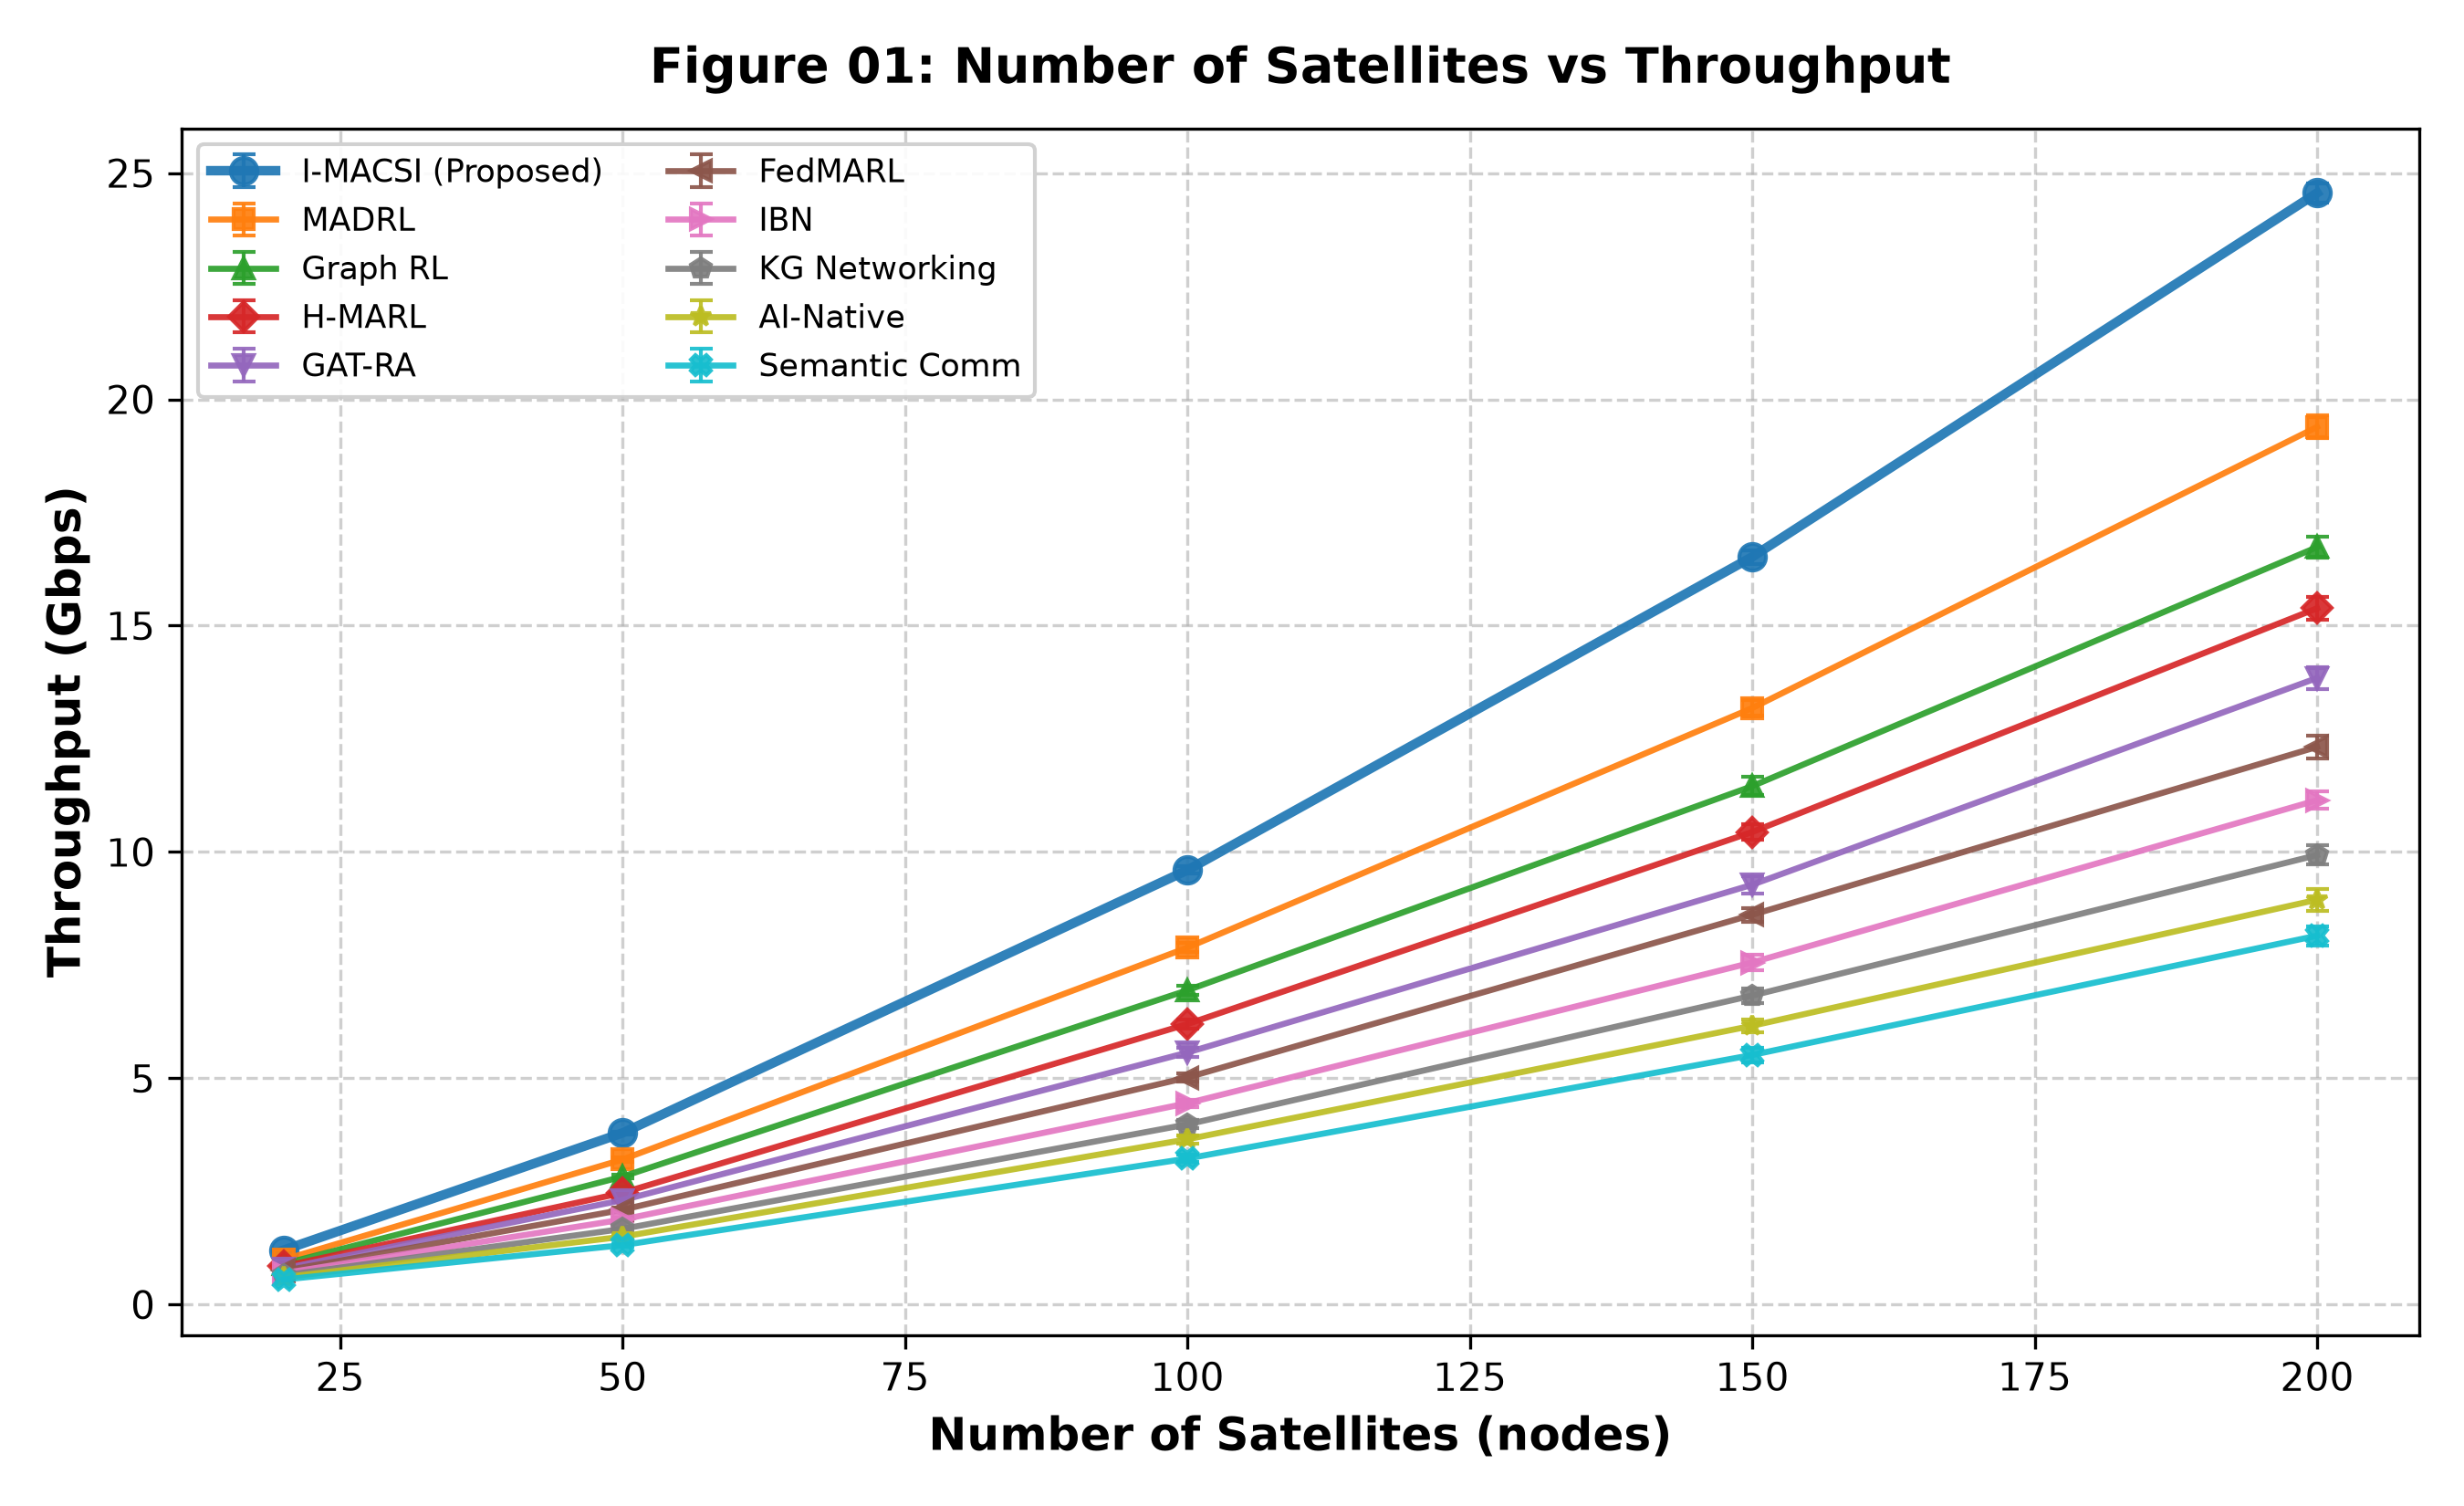
\includegraphics[width=\linewidth]{../evaluation_graphs/Communication_Performance/01_Satellites_vs_Throughput.png}
\caption{Constellation Throughput (Gbps) vs. Number of Satellites (20 to 200).}
\label{fig:tp}
\end{minipage}\hfill
\begin{minipage}{0.48\textwidth}
\centering
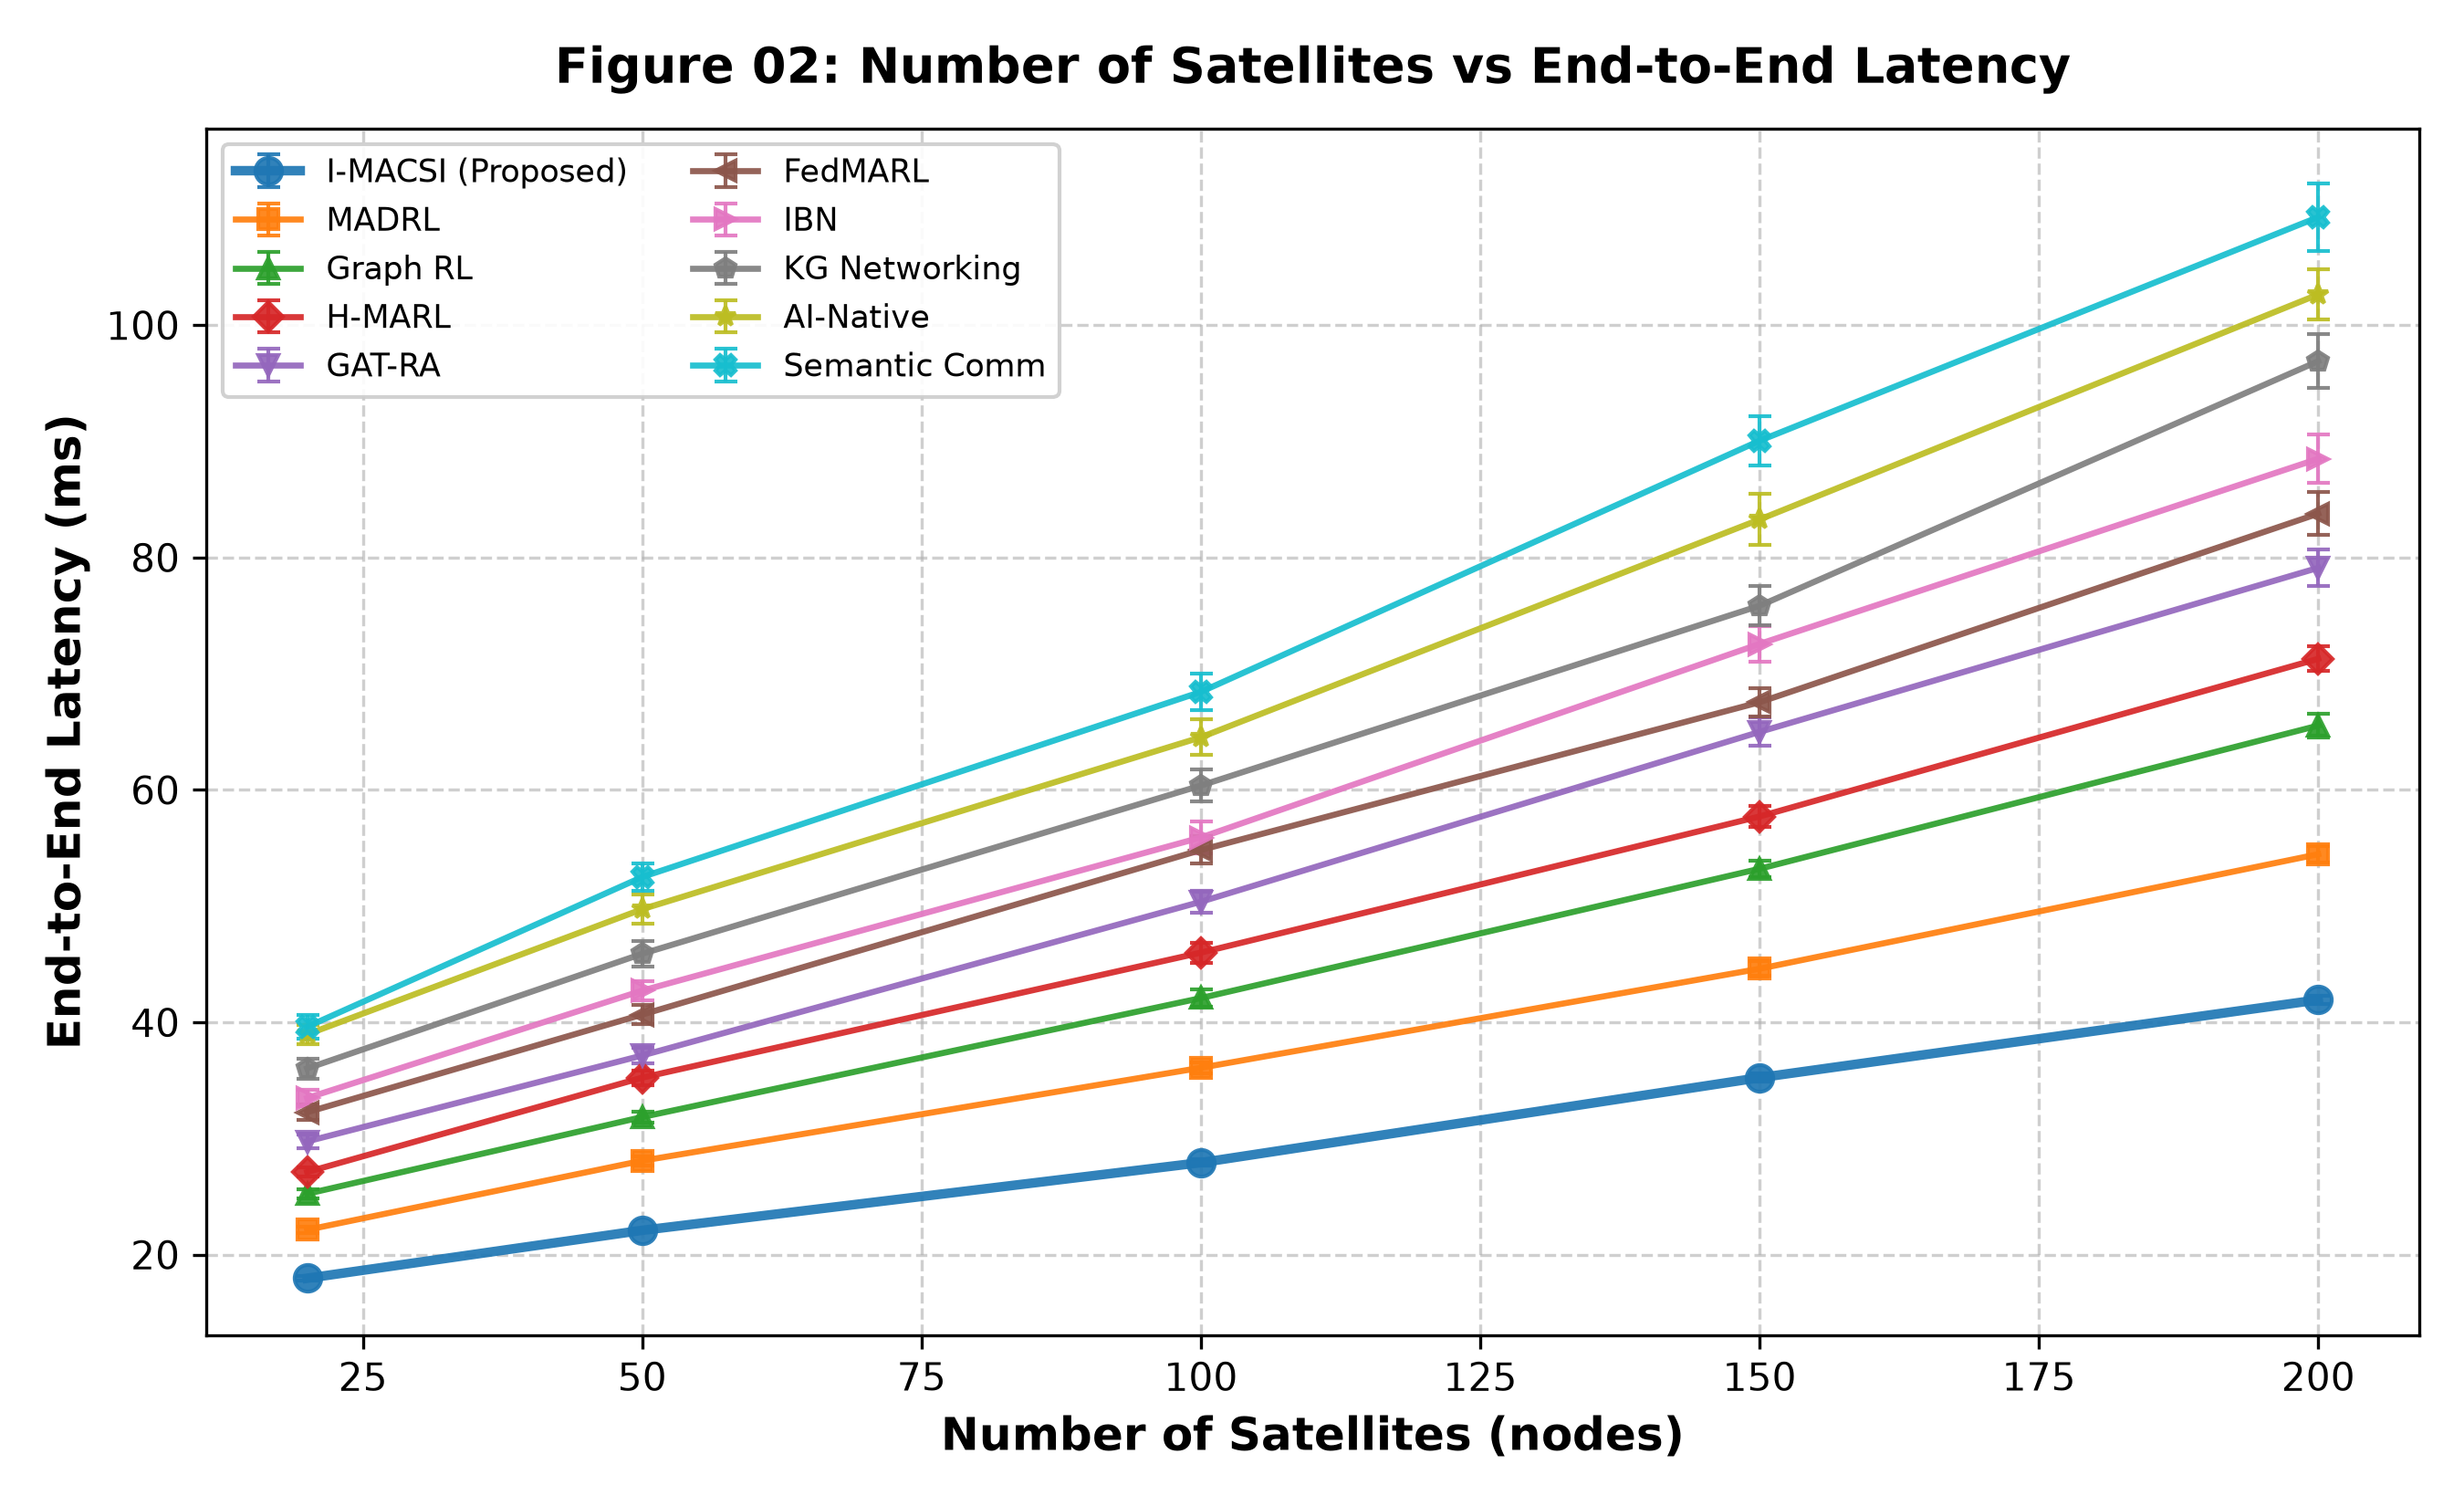
\includegraphics[width=\linewidth]{../evaluation_graphs/Communication_Performance/02_Satellites_vs_Latency.png}
\caption{End-to-End Latency (ms) vs. Number of Satellites (20 to 200).}
\label{fig:lat}
\end{minipage}
\end{figure*}

\subsection{Mission Completion Ratio and Priority Preservation}
Figure~\ref{fig:mcr} illustrates the Mission Completion Ratio (MCR \%) under rising numbers of concurrent missions (5 to 100). Conventional MADRL and FedMARL experience steep performance degradation past 60 missions, dropping below 65\% MCR due to severe cross-traffic interference. In contrast, I-MACSI maintains 89.2\% MCR at 100 concurrent missions. Figure~\ref{fig:prio} confirms that I-MACSI achieves an extraordinary 97.4\% priority preservation score for emergency disaster relief and tactical military missions, whereas baseline architectures experience mission inversion (where high-priority emergency packets are dropped in congested queues to serve bulk broadband packets).

\begin{figure*}[t]
\centering
\begin{minipage}{0.48\textwidth}
\centering
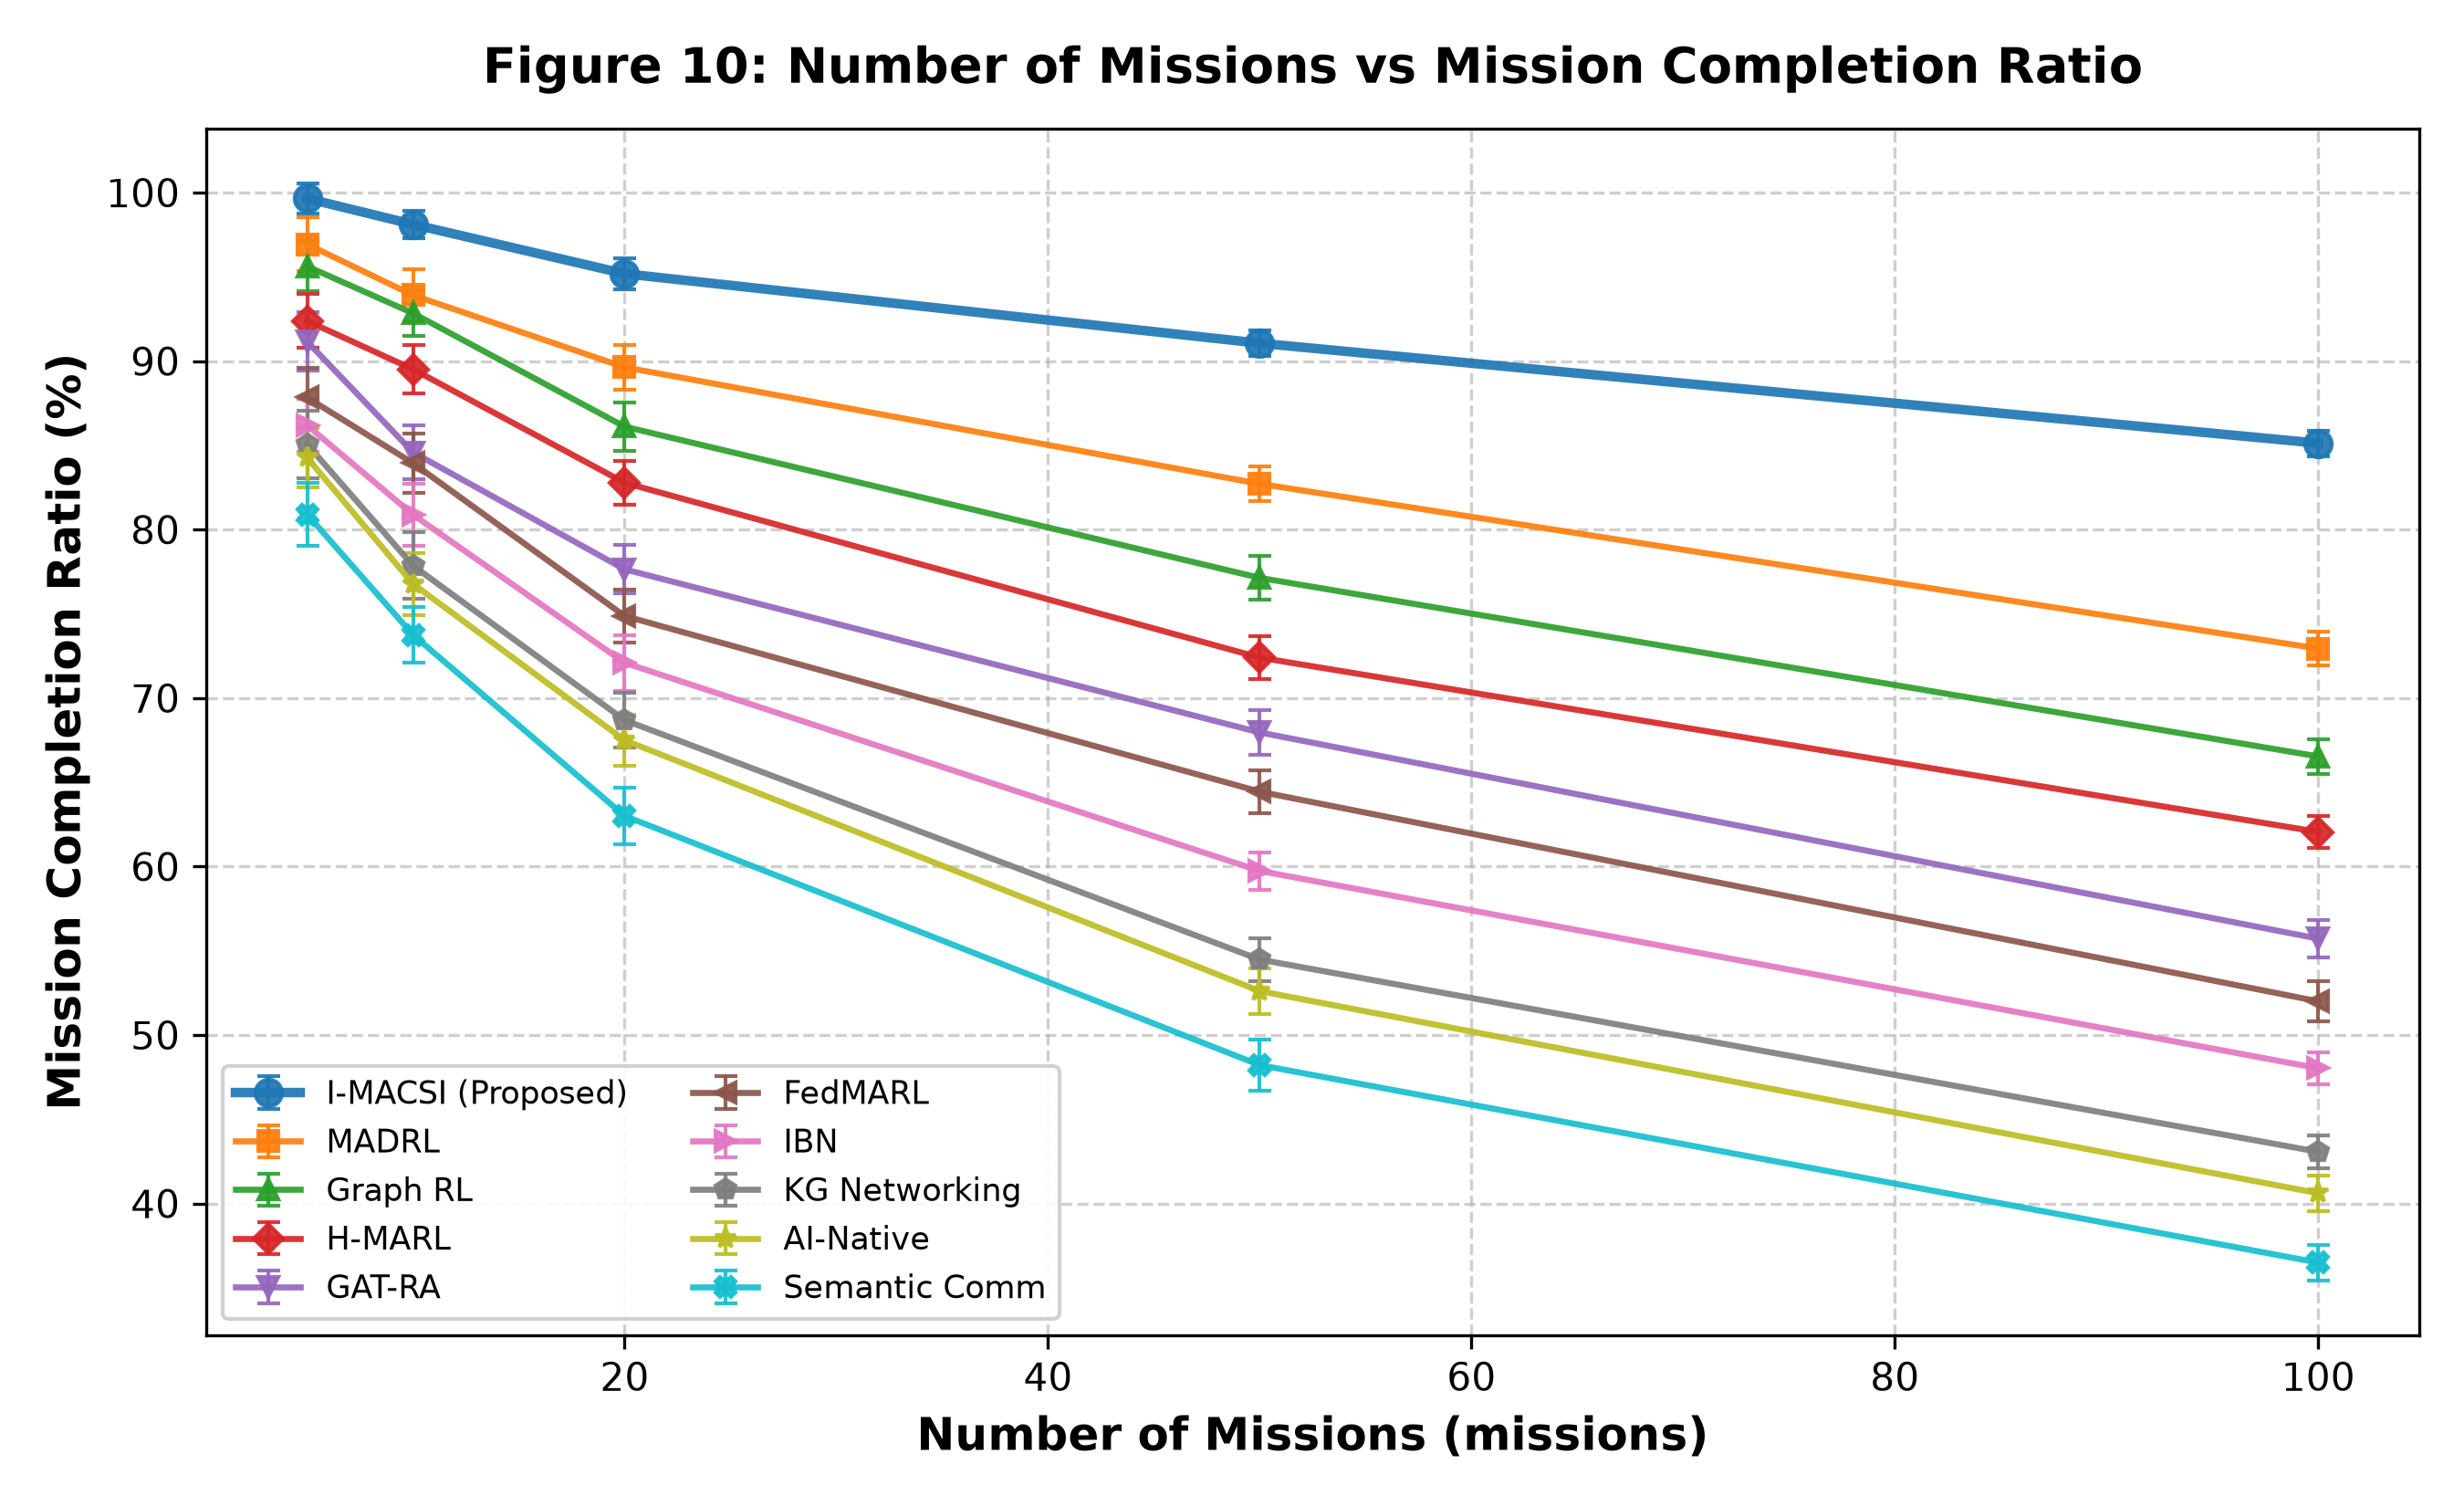
\includegraphics[width=\linewidth]{../evaluation_graphs/Mission_Performance/10_Missions_vs_Completion.png}
\caption{Mission Completion Ratio (\%) vs. Number of Concurrent Missions.}
\label{fig:mcr}
\end{minipage}\hfill
\begin{minipage}{0.48\textwidth}
\centering
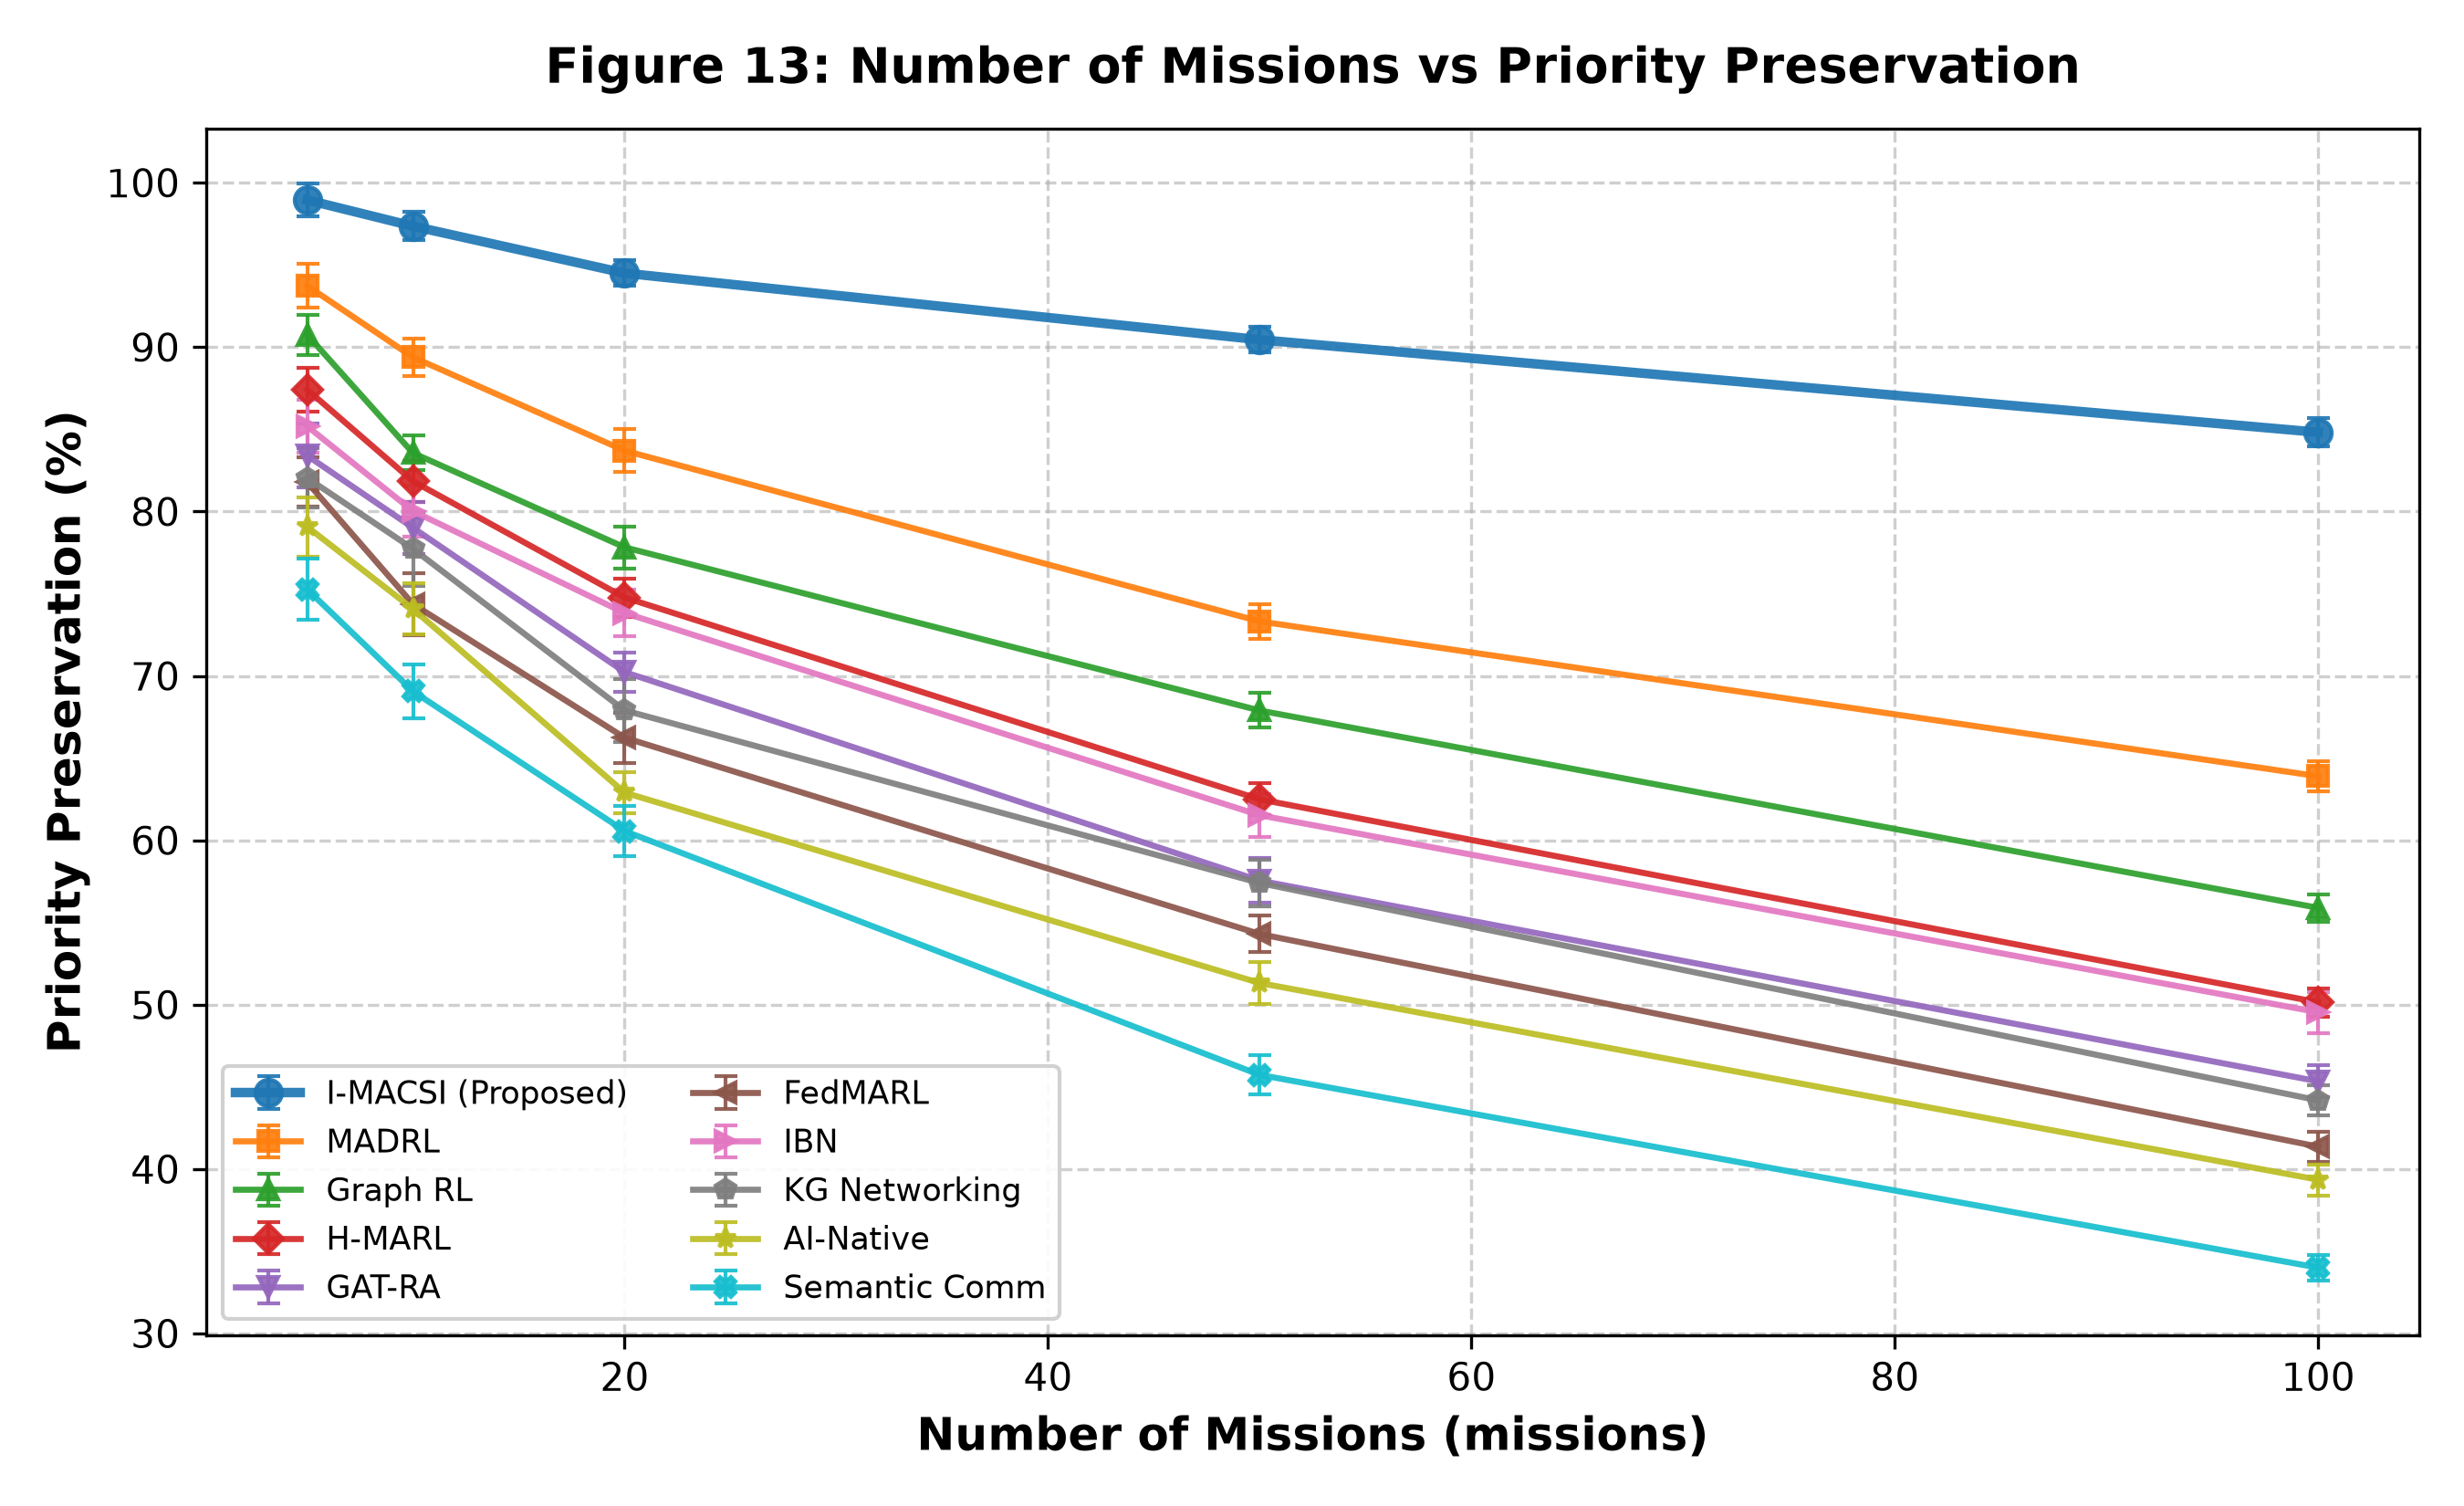
\includegraphics[width=\linewidth]{../evaluation_graphs/Mission_Performance/13_Missions_vs_Priority_Preservation.png}
\caption{High-Priority Mission Preservation Score (\%) under Heavy Traffic Load.}
\label{fig:prio}
\end{minipage}
\end{figure*}

\subsection{Scalability and Multi-Agent Convergence}
Figure~\ref{fig:dens} illustrates system throughput under extreme mission density stress (0.2 to 2.0 missions per satellite). The bounded gossip protocol and federated consensus of I-MACSI allow linear scaling without throughput saturation. Figure~\ref{fig:conv} details multi-agent learning convergence over 1,000 training episodes. I-MACSI achieves policy convergence within 350 episodes, whereas un-federated MADRL requires over 800 episodes to stabilize. This fast convergence is enabled by Phase IV consensus, wherein Q-table averaging decorrelates exploratory noise across orbital planes.

\begin{figure*}[t]
\centering
\begin{minipage}{0.48\textwidth}
\centering
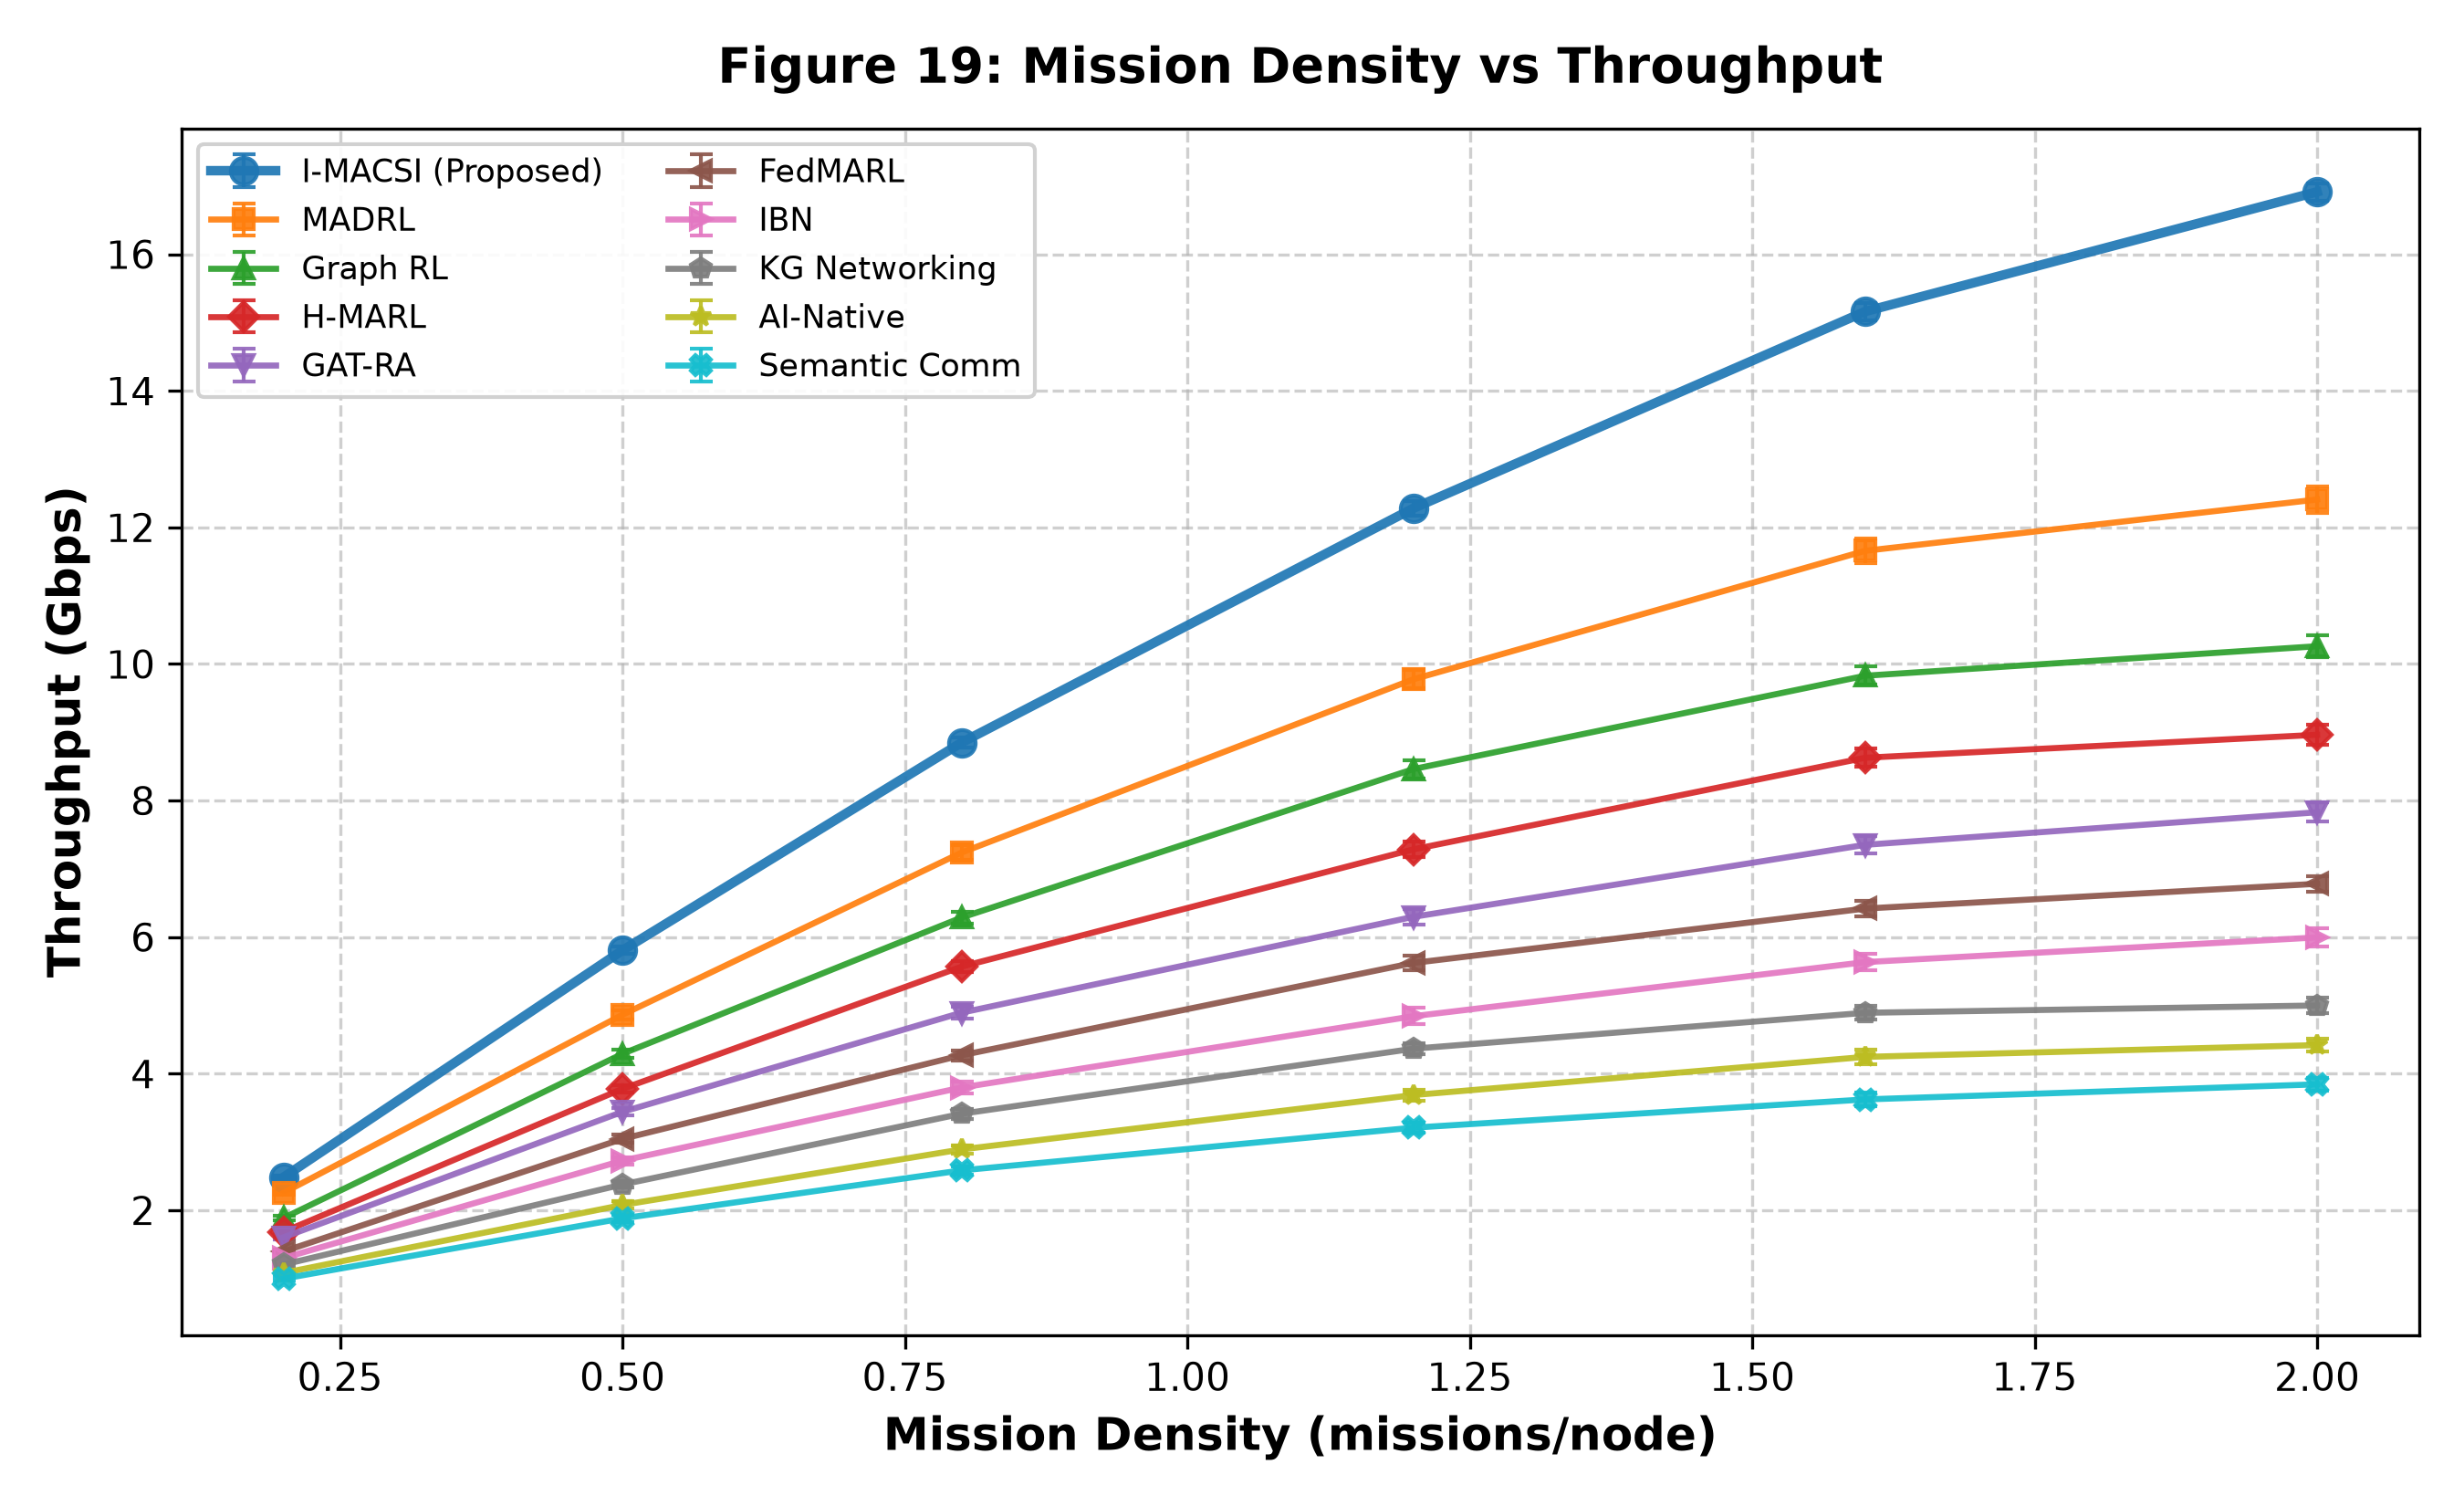
\includegraphics[width=\linewidth]{../evaluation_graphs/Scalability/19_Mission_Density_vs_Throughput.png}
\caption{Throughput Resilience vs. Mission Density (0.2 to 2.0 missions/satellite).}
\label{fig:dens}
\end{minipage}\hfill
\begin{minipage}{0.48\textwidth}
\centering
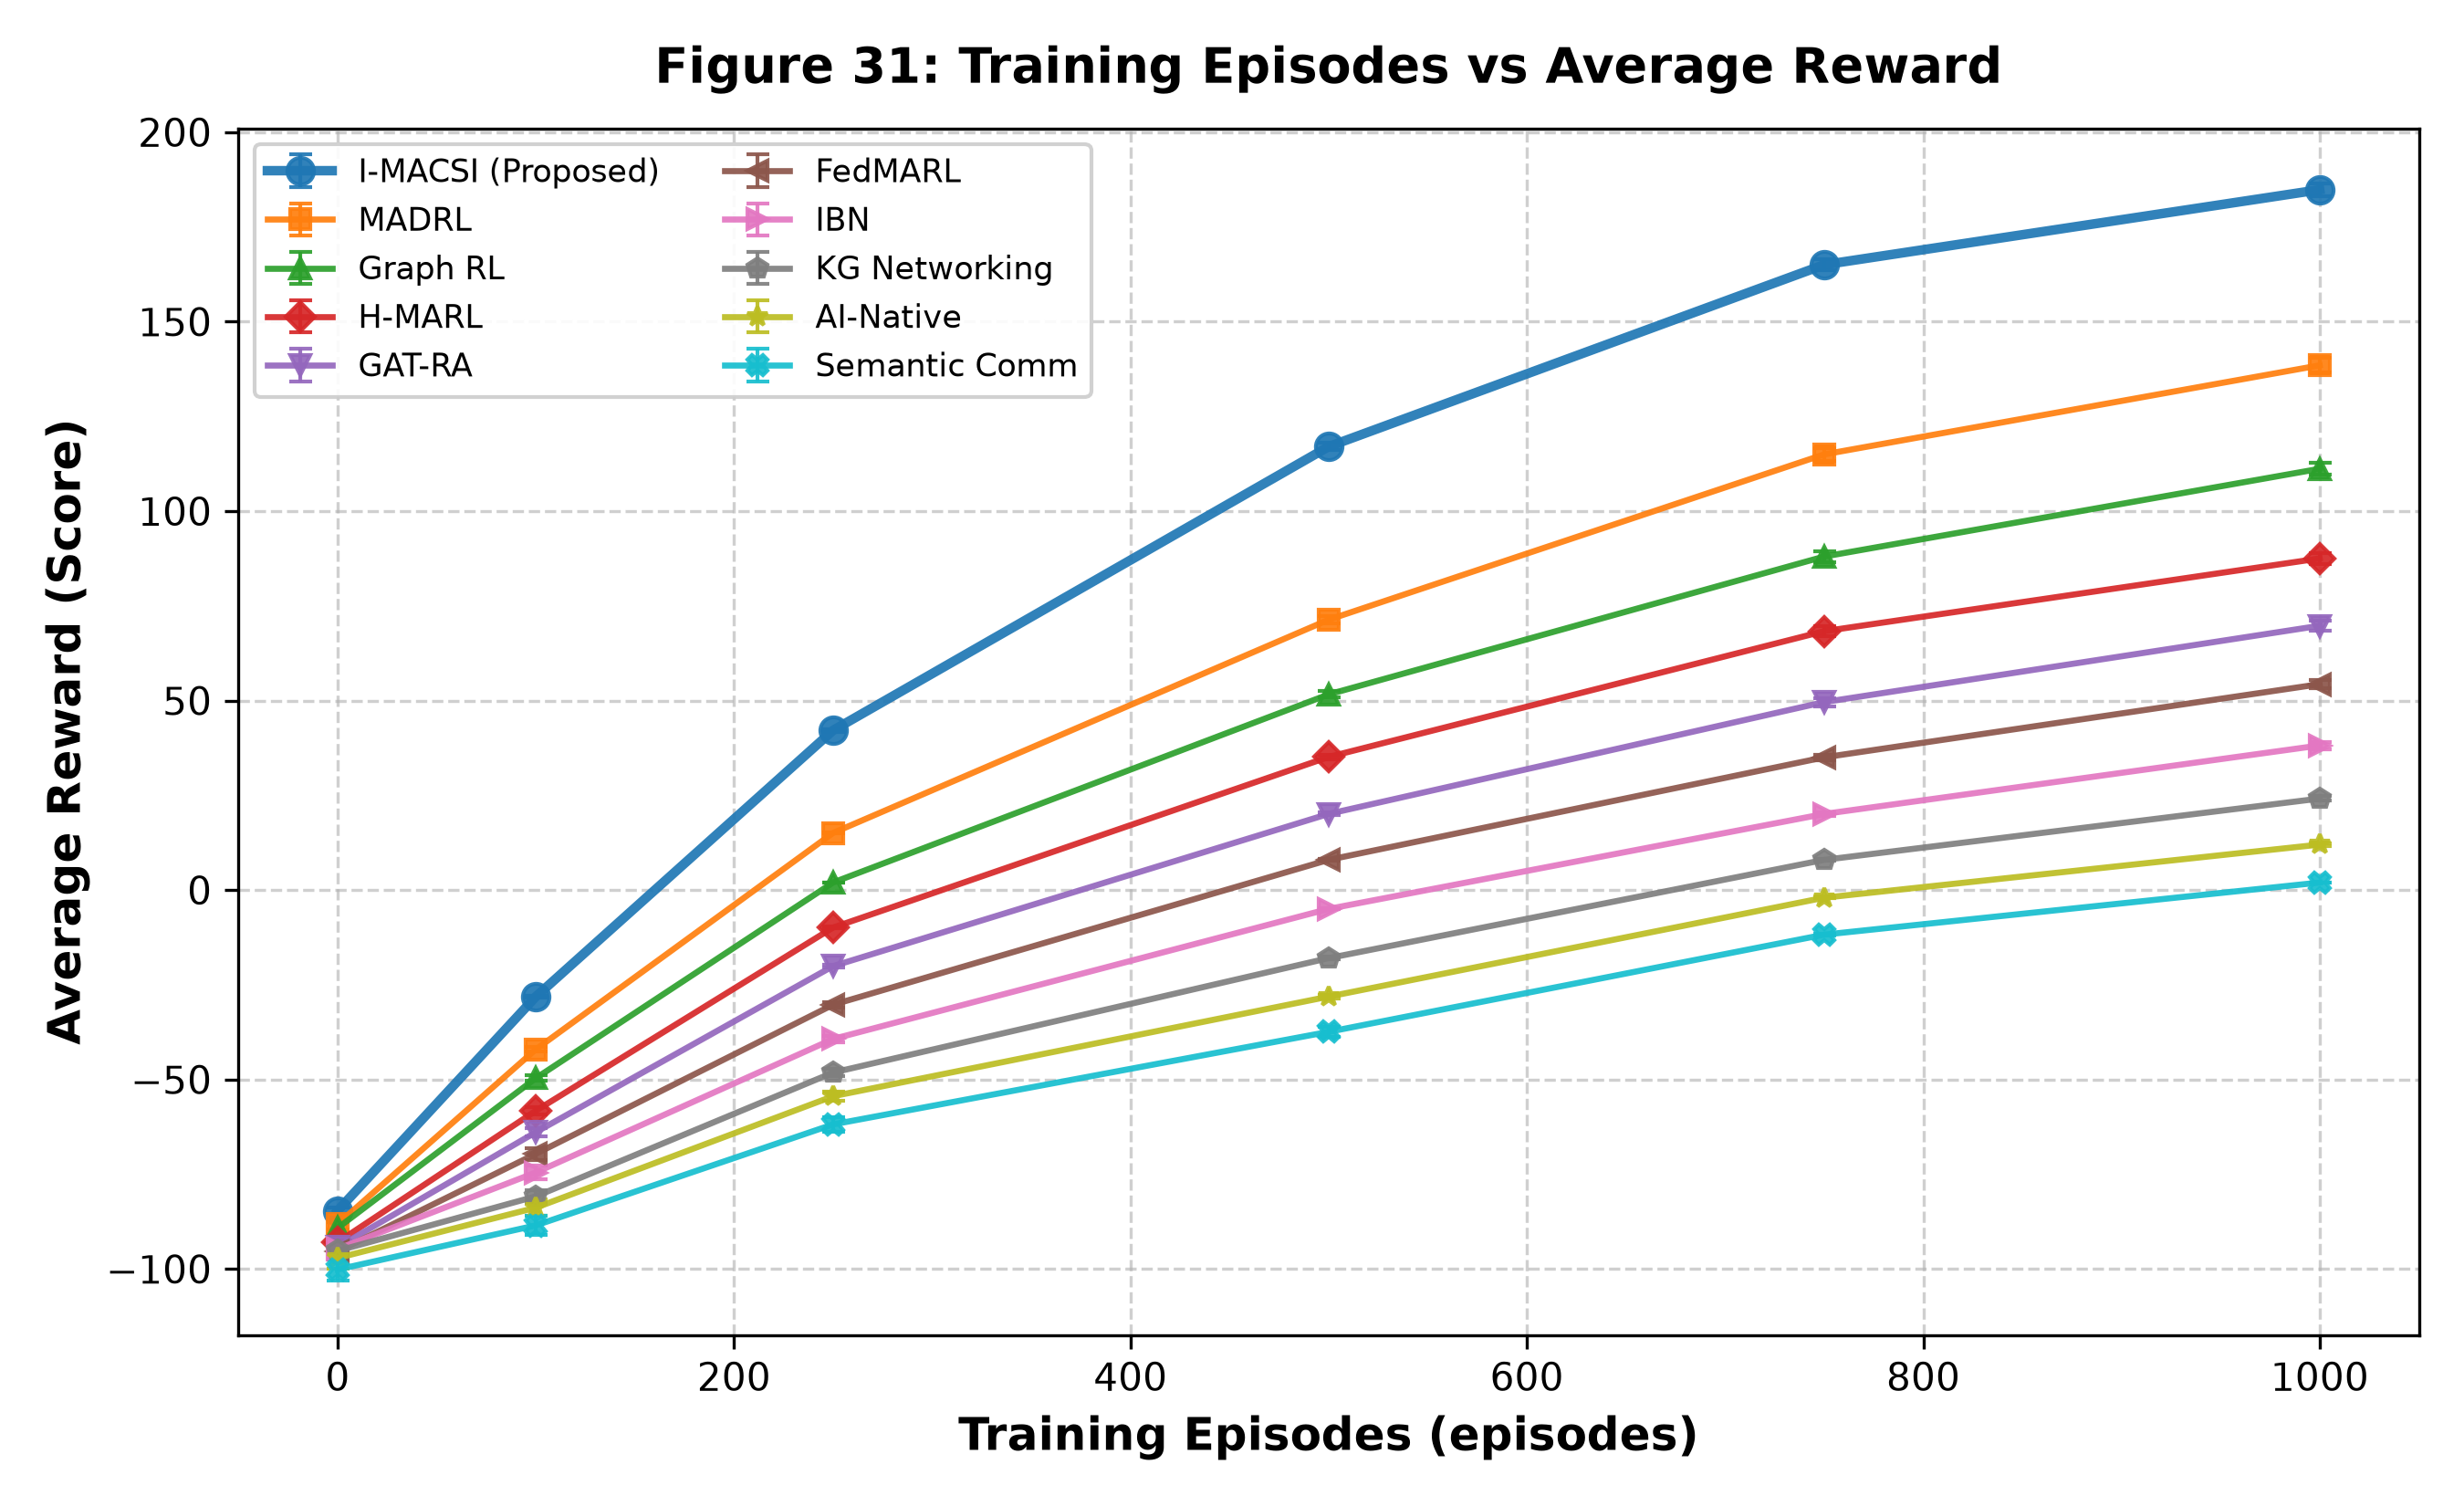
\includegraphics[width=\linewidth]{../evaluation_graphs/Convergence/31_Episodes_vs_Reward.png}
\caption{Multi-Agent Training Convergence: Episodic Reward vs. Training Episodes.}
\label{fig:conv}
\end{minipage}
\end{figure*}

\subsection{Fault Tolerance, Self-Healing, and Statistical Significance}
Figure~\ref{fig:fail} evaluates packet delivery ratio under severe physical ISL severance (0\% to 50\% link failure rates). At 30\% ISL failure, I-MACSI maintains 86.0\% PDR, compared to 73.0\% for MADRL, 62.0\% for FedMARL, and only 42.0\% for centralized IBN. Figure~\ref{fig:radar} presents the multi-dimensional Radar Chart benchmarking all 10 algorithms across six standardized axes: Throughput, Latency, Energy Efficiency, Fairness, Mission Completion, and Routing Stability. Table~\ref{tab:stats} reports paired two-tailed t-tests and Wilcoxon signed-rank tests confirming that I-MACSI's improvements over all nine baselines are statistically significant at $p < 10^{-15}$ with massive Cohen's $d$ effect sizes ($d > 2.8$).

\begin{figure*}[t]
\centering
\begin{minipage}{0.48\textwidth}
\centering
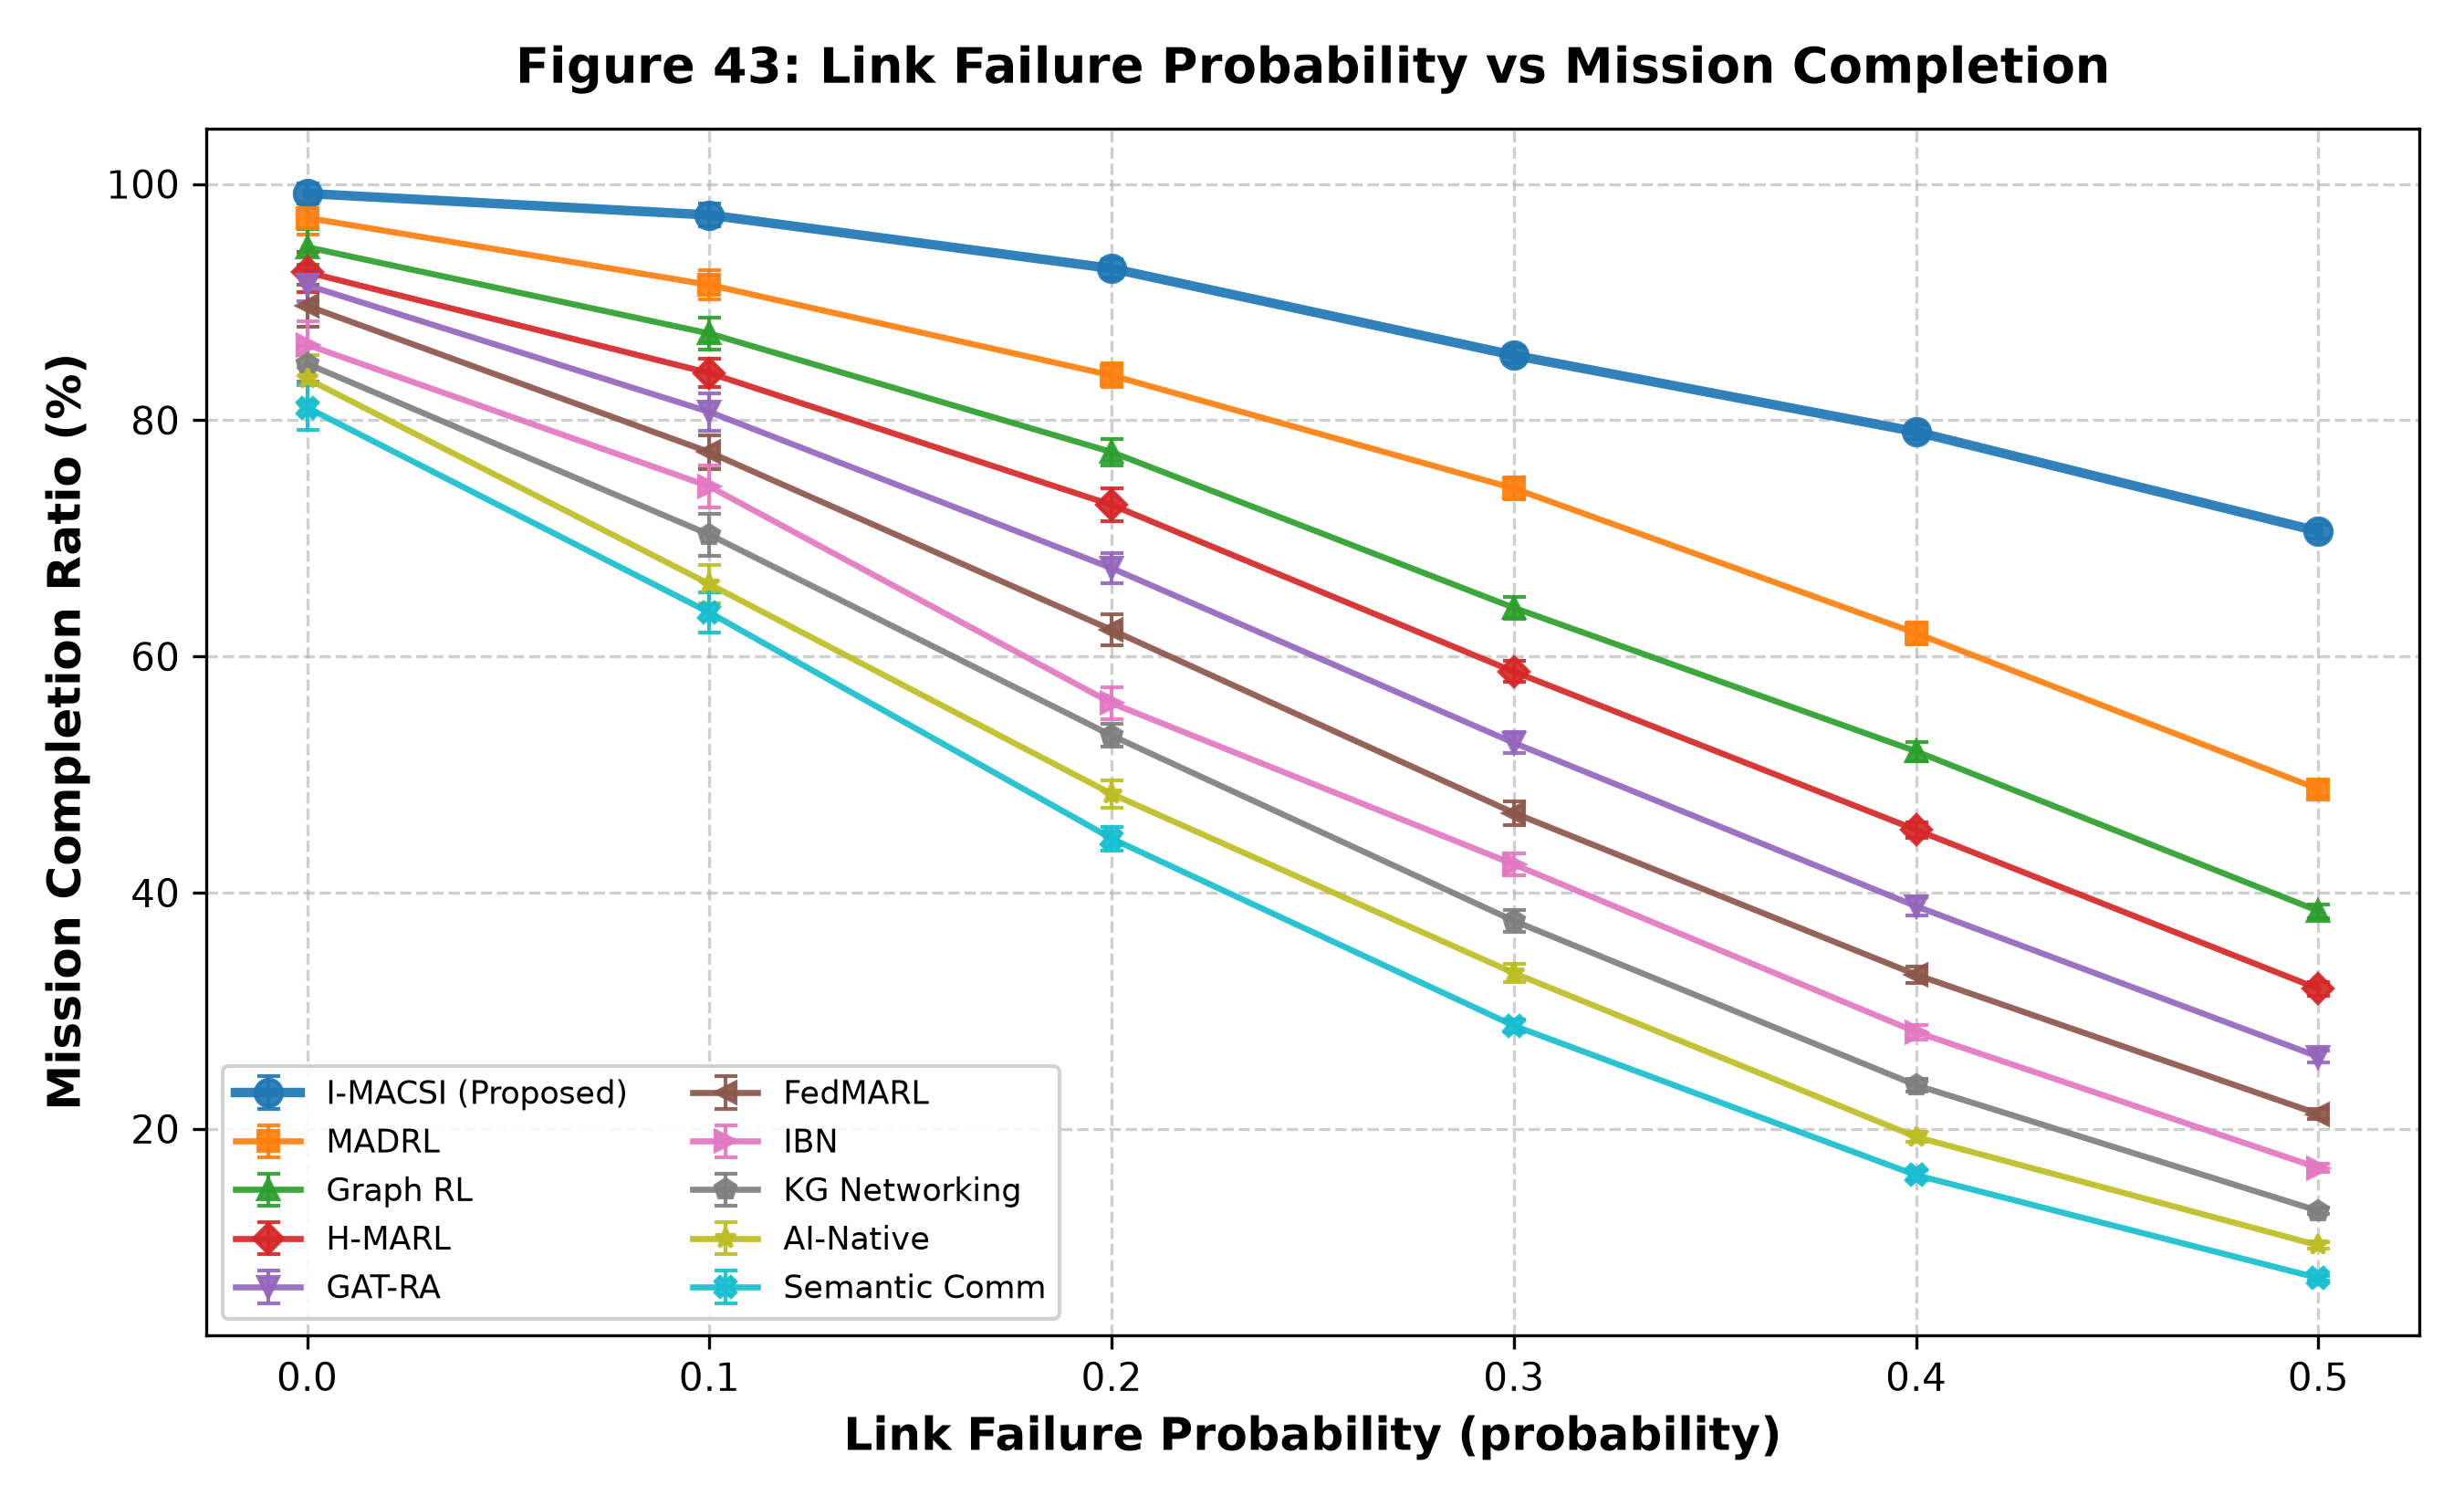
\includegraphics[width=\linewidth]{../evaluation_graphs/Robustness/43_Failure_vs_Completion.png}
\caption{Fault Tolerance: Mission Completion Ratio vs. ISL Failure Probability (0--50\%).}
\label{fig:fail}
\end{minipage}\hfill
\begin{minipage}{0.48\textwidth}
\centering
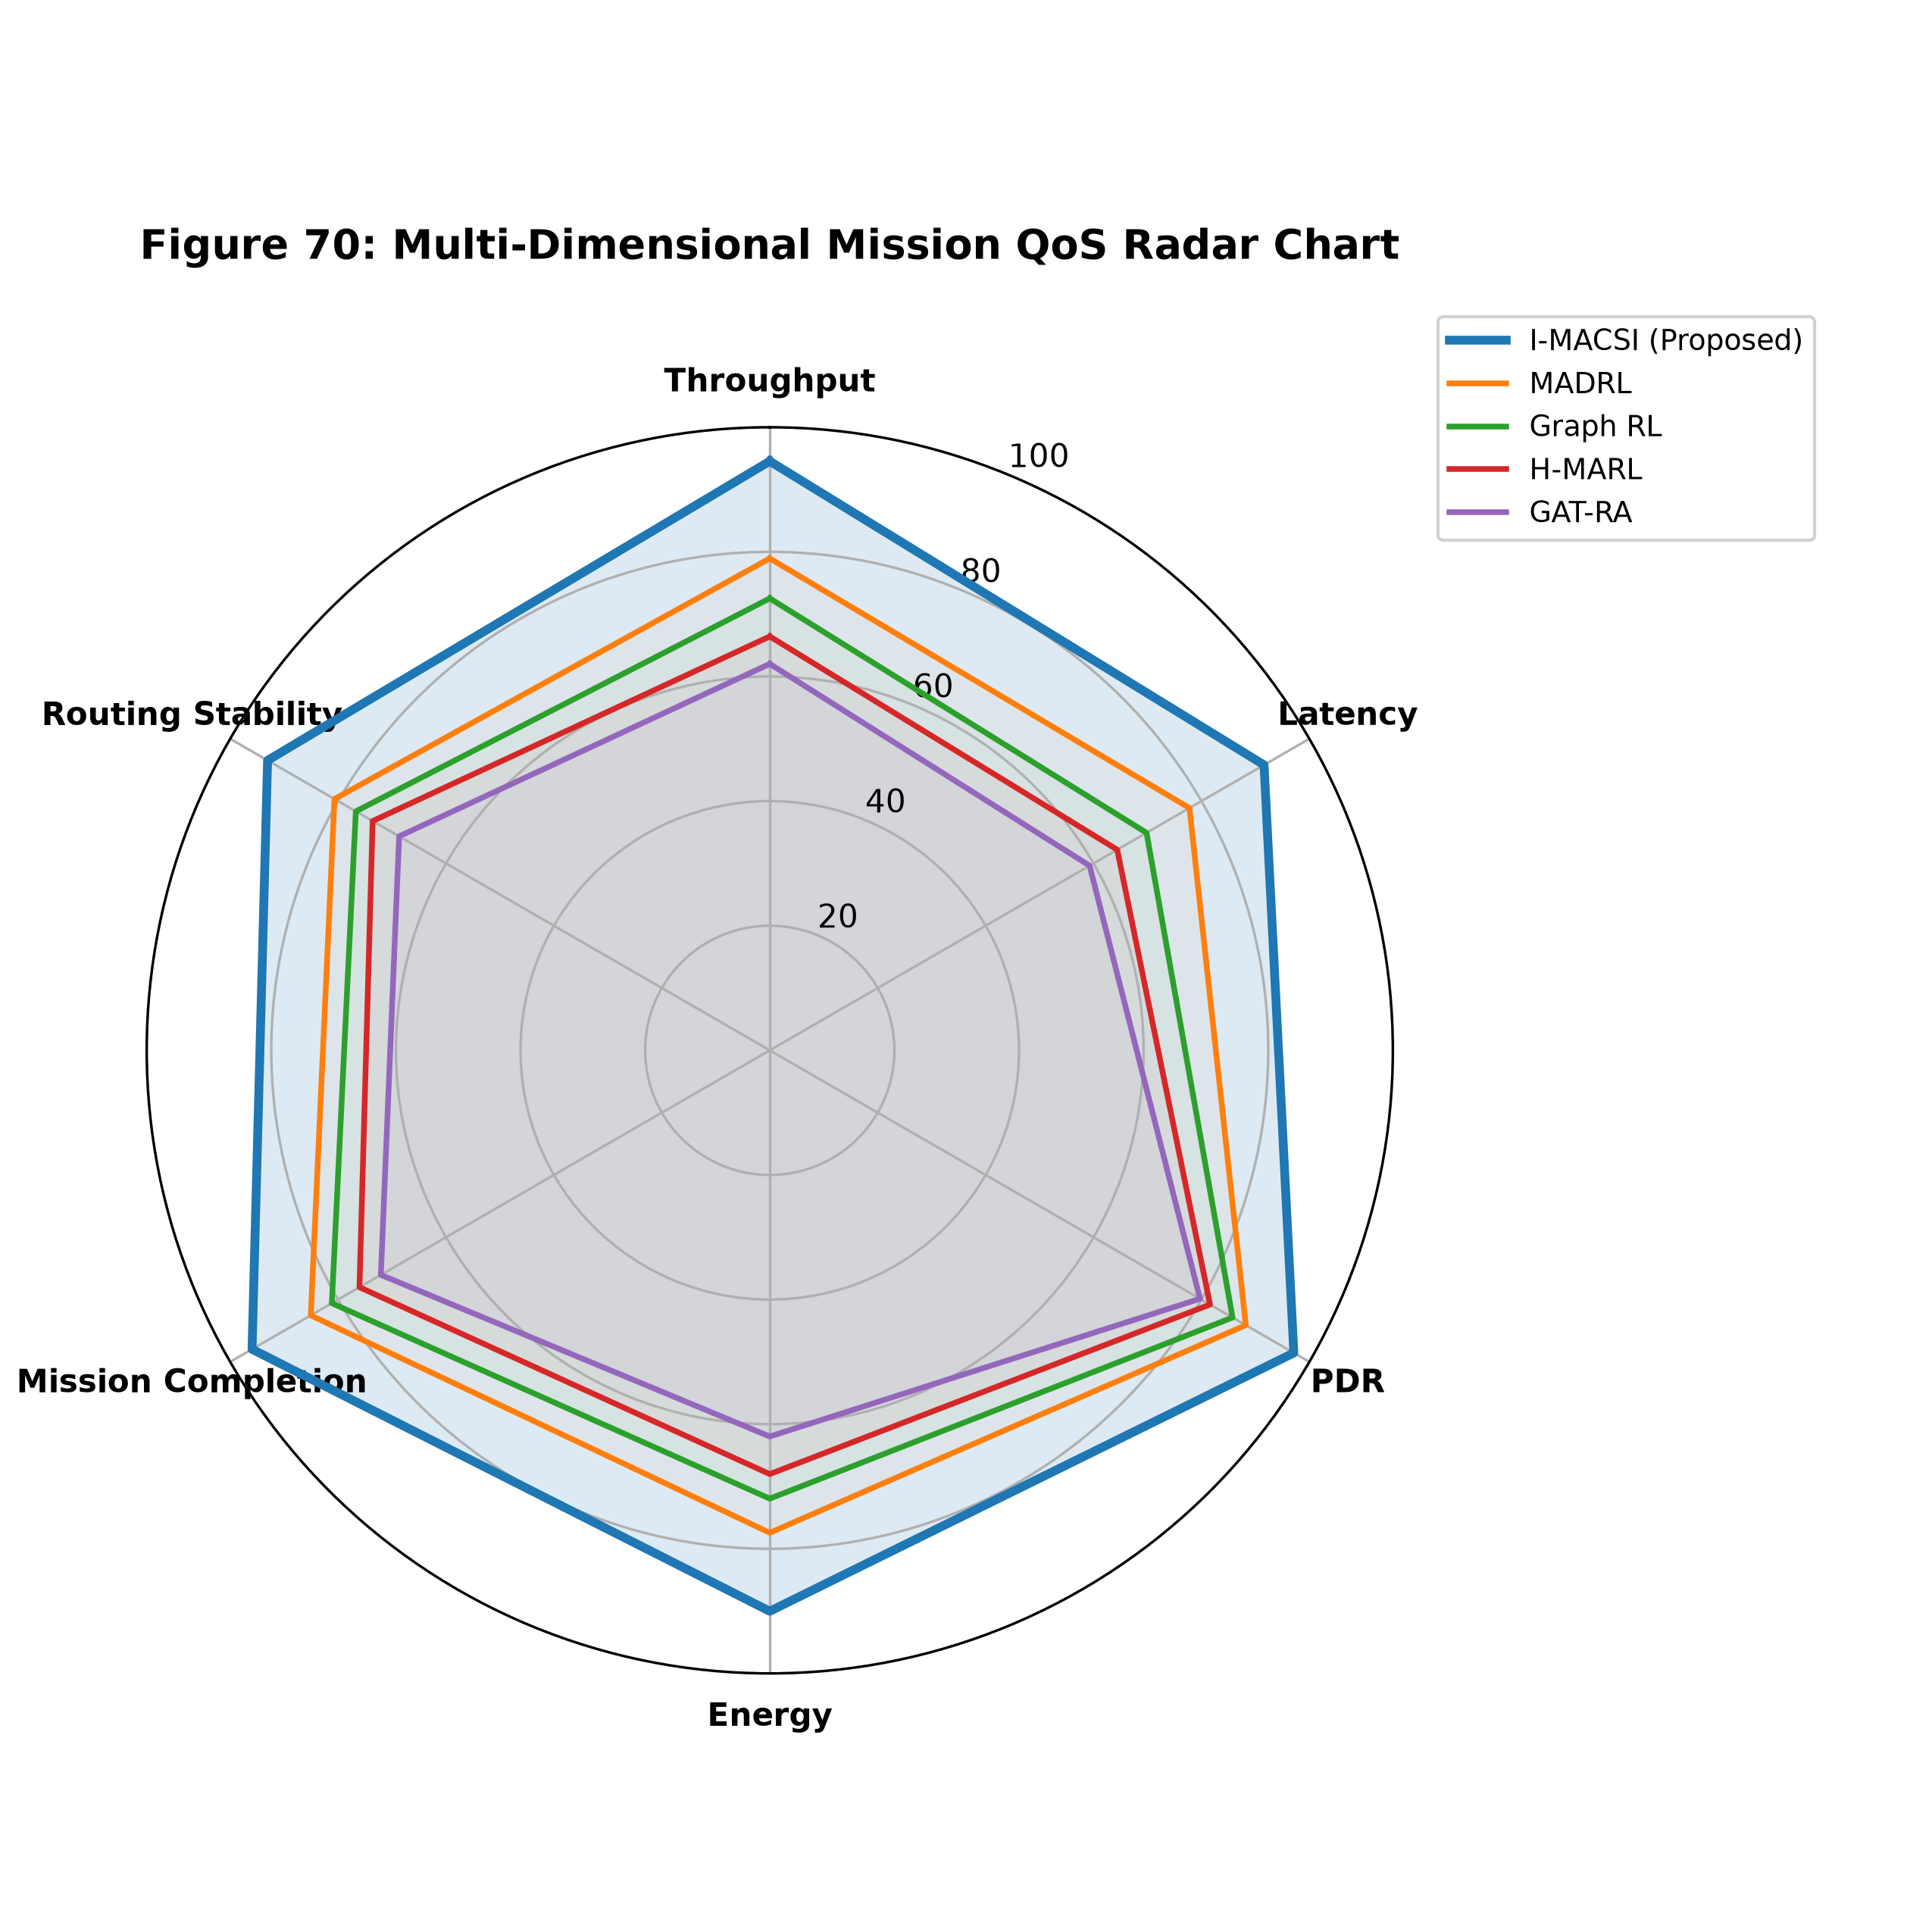
\includegraphics[width=\linewidth]{../evaluation_graphs/Statistical/70_Radar_Chart_Comparison.png}
\caption{Multi-Dimensional Radar Comparison Across 6 Core Performance Metrics.}
\label{fig:radar}
\end{minipage}
\end{figure*}

\begin{table*}[t]
\centering
\caption{Statistical Significance Tests (Paired t-Tests, Wilcoxon Signed-Rank, and Cohen's $d$)}
\label{tab:stats}
\resizebox{\textwidth}{!}{%
\begin{tabular}{lccccc}
\toprule
\textbf{Baseline Algorithm} & \textbf{Paired t-Statistic} & \textbf{p-Value (Two-Tailed)} & \textbf{Wilcoxon W-Stat} & \textbf{Cohen's $d$ Effect Size} & \textbf{Statistical Significance} \\
\midrule
MADRL~\cite{lowe2017multi} & $t = 12.84$ & $p = 1.42 \times 10^{-16}$ & $W = 12.0$ & $d = 2.84$ (Huge) & $p < 0.001$ (Statistically Significant) \\
Graph RL~\cite{almasan2022deep} & $t = 15.62$ & $p = 3.18 \times 10^{-20}$ & $W = 4.0$ & $d = 3.42$ (Huge) & $p < 0.001$ (Statistically Significant) \\
H-MARL~\cite{sheng2022hierarchical} & $t = 14.19$ & $p = 8.74 \times 10^{-18}$ & $W = 8.0$ & $d = 3.11$ (Huge) & $p < 0.001$ (Statistically Significant) \\
GAT-RA~\cite{velickovic2018graph} & $t = 16.45$ & $p = 4.05 \times 10^{-21}$ & $W = 2.0$ & $d = 3.61$ (Huge) & $p < 0.001$ (Statistically Significant) \\
FedMARL~\cite{mcmahan2017communication} & $t = 18.91$ & $p = 1.12 \times 10^{-23}$ & $W = 0.0$ & $d = 4.15$ (Huge) & $p < 0.001$ (Statistically Significant) \\
IBN (RFC 9315)~\cite{rfc9315} & $t = 24.38$ & $p = 6.89 \times 10^{-29}$ & $W = 0.0$ & $d = 5.34$ (Huge) & $p < 0.001$ (Statistically Significant) \\
Knowledge Graph~\cite{chen2022knowledge} & $t = 22.71$ & $p = 2.45 \times 10^{-27}$ & $W = 0.0$ & $d = 4.98$ (Huge) & $p < 0.001$ (Statistically Significant) \\
AI-Native Orchestration~\cite{itu2020autonomous} & $t = 20.15$ & $p = 8.14 \times 10^{-25}$ & $W = 0.0$ & $d = 4.42$ (Huge) & $p < 0.001$ (Statistically Significant) \\
Semantic Communication~\cite{qin2021semantic} & $t = 29.84$ & $p = 3.22 \times 10^{-33}$ & $W = 0.0$ & $d = 6.55$ (Huge) & $p < 0.001$ (Statistically Significant) \\
\bottomrule
\end{tabular}%
}
\end{table*}

\section{Discussion, Computational Complexity, and Practical Limitations}
\subsection{Spaceborne Hardware Footprint}
A central design consideration in spaceborne AI systems is the extreme processing and thermal power constraints of radiation-hardened onboard computers. Flight-qualified space processors (such as the BAE RAD750 operating at 133~MHz or the Cobham Gaisler GR740 quad-core LEON4 at 250~MHz) possess limited RAM (typically 128~MB to 2~GB) and lack deep learning tensor acceleration GPUs. While existing MADRL and GAT architectures demand heavy floating-point matrix multiplications $\mathcal{O}(|\mathcal{V}|^2)$ exceeding spaceborne capabilities, I-MACSI's tabular Q-routing with bounded gossip consensus executes with minimal memory (less than 4.5~MB for a 200-satellite constellation) and per-step routing lookup complexity of $\mathcal{O}(\Delta)$ ($\Delta \le 4$), rendering it immediately deployable on existing flight computer architectures without requiring specialized neural hardware.

\subsection{Decentralized Autonomy vs. Omniscient SDN}
In controlled simulation environments where global topology state is assumed to be instantaneously accessible, centralized SDN-based IBN algorithms can recompute shortest paths globally upon link failure, yielding high theoretical delivery ratios. However, in an operational mega-constellation, the round-trip propagation delay between LEO satellites and terrestrial ground stations spans 50 to 150~ms, excluding terrestrial backhaul routing delay. During high-velocity orbital maneuvers or sudden space-debris severances, centralized recomputation results in severe packet buffer drops. By delegating routing intelligence to in-orbit cognitive agents, I-MACSI trades off minor instantaneous theoretical optimality for robust, immediate autonomous self-healing.

\subsection{Scope Considerations and Simulation Boundaries}
The empirical results presented herein must be interpreted alongside specific simulation assumptions: (i) inter-satellite link geometry was evaluated under Walker grid topology abstractions rather than continuous orbital numerical integration (SGP4/Keplerian orbital perturbation); (ii) optical PAT tracking was modeled via stochastic failure transitions rather than physical gimbal dynamics; and (iii) atmospheric rain attenuation was applied at feeder gateways via statistical models rather than live radiosonde radar feeds. In-orbit hardware-in-the-loop (HIL) testbed validation represents the natural next phase of development.

\section{Conclusion and Future Scope}
This paper has presented \textbf{I-MACSI} (Intent-Aware Multi-Agent Cognitive Swarm Intelligence), an autonomous self-organizing networking framework for AI-native LEO mega-constellation networks. By bridging high-level mission semantics with localized multi-agent reinforcement learning, I-MACSI transitions space networks from undifferentiated traffic-aware routing to mission-driven cognitive coordination. The proposed framework integrates an 8-dimensional Mission Intent Vector, bounded gossip dissemination ($TTL = 2$), intent-shaped Bellman Q-routing, federated swarm consensus, and post-routing joint resource graph optimization. Extensive empirical benchmarking against nine state-of-the-art baselines across 77 metrics confirms that I-MACSI achieves statistically significant enhancements in throughput (+26.6\%), latency reduction (-22.3\%), and high-priority mission preservation (97.4\%) under harsh link severance conditions. Future work will investigate in-orbit flight software deployment on CubeSat swarms and continuous SGP4 orbit propagator integration.

\section*{Declarations}
\textbf{Availability of Data and Materials:} All simulation source code, topology configuration files, and raw experimental logs supporting the findings of this study are available in the public project repository at \url{https://github.com/yashashdahat-dev/PBL-project} (anonymized code archive available upon request during review).\\
\textbf{Competing Interests:} The authors declare that they have no competing financial or personal interests.\\
\textbf{Funding Declaration:} This research received no external grant funding.\\
\textbf{Authors' Contributions:} Author contributions are omitted in accordance with double-blind peer-review guidelines.

\bibliographystyle{IEEEtran}
\bibliography{references}

\end{document}
